% ─────────────────────────────────────────────────────────────────────────────
\chapter{Methodology}
\label{chap:methodology}
% ─────────────────────────────────────────────────────────────────────────────

This chapter defines the methodology adopted to evaluate the operational
robustness of \gls{ai}-based tools for automated image classification in
forensic contexts. It addresses the gap identified in
Chapter~\ref{chap:state-of-the-art} by formalizing the \gls{fairlab} framework
as a reproducible and auditable protocol that combines controlled experimental
conditions with operationally relevant forensic scenarios.

The chapter presents the overall framework and research assumptions, followed
by the procedures for dataset construction, human-in-the-loop validation,
dataset freezing and partitioning, proxy-model and black-box software
evaluation, perturbation testing, metric computation, explainability, and
traceability. Implementation-specific data structures, scripts, architectures,
parameters, software versions, and configurations are documented in
Chapter~\ref{chap:implementation}; quantitative outcomes and their
interpretation are reported in Chapter~\ref{chap:results}.

% ─────────────────────────────────────────────────────────────────────────────
\section{Overview of the FAIRLab Methodology}
\label{sec:methodology-fairlab-overview}
% ─────────────────────────────────────────────────────────────────────────────

The \gls{fairlab} protocol provides a structured framework for evaluating
automated image-classification systems under clean, \gls{ood}, adversarial,
and anti-forensic conditions. Its scope extends beyond clean classification
accuracy because automated outputs may affect evidence prioritization and the
allocation of human analytical resources. Operational robustness is therefore
examined in relation to missed relevant content, additional review workload,
and unstable behavior on inputs that differ from the expected operational
distribution.

The protocol integrates two complementary evaluation levels. The first uses
fully inspectable proxy classification models as controlled experimental
references; these models are not treated as replicas or functionally equivalent
substitutes for proprietary systems. The second evaluates selected
\gls{ai}-based software systems under black-box or near-black-box access
conditions, using only their observable inputs and outputs and making no
assumptions about inaccessible architectures, training data, calibration
procedures, or decision logic
\cite{sanna2024preliminary,sanna2025pixelperfect}.

Both levels rely on the same frozen experimental corpus. Its binary in-domain
component supports clean and perturbed evaluation, whereas a separate clean
\gls{ood} branch is evaluated outside model training and perturbation
generation, as detailed in
Section~\ref{sec:methodology-split-generation}. The clean binary samples,
clean \gls{ood} inputs, adversarial artifacts, and anti-forensic artifacts are
combined into a common evaluation bundle, enabling comparison under aligned
experimental conditions.

Quantitative metrics characterize classification performance, robustness
degradation, error direction, and \gls{ood} behavior. Explainability provides
qualitative diagnostic evidence for selected cases involving an inspectable
proxy model and is not extended to the selected black-box systems.
Traceability controls preserve the relationships among source samples, derived
artifacts, experimental conditions, observable outputs, and reported results.

The protocol specifies the methodological requirements and information that
must be preserved without prescribing particular model architectures, software
products, file formats, directory structures, databases, hashing algorithms,
or explainability techniques. These choices belong to the concrete
implementation documented in Chapter~\ref{chap:implementation}.
Figure~\ref{fig:methodology-fairlab-overview} summarizes the resulting
workflow.




\begin{figure}[H]
\centering
\resizebox{\textwidth}{!}{%
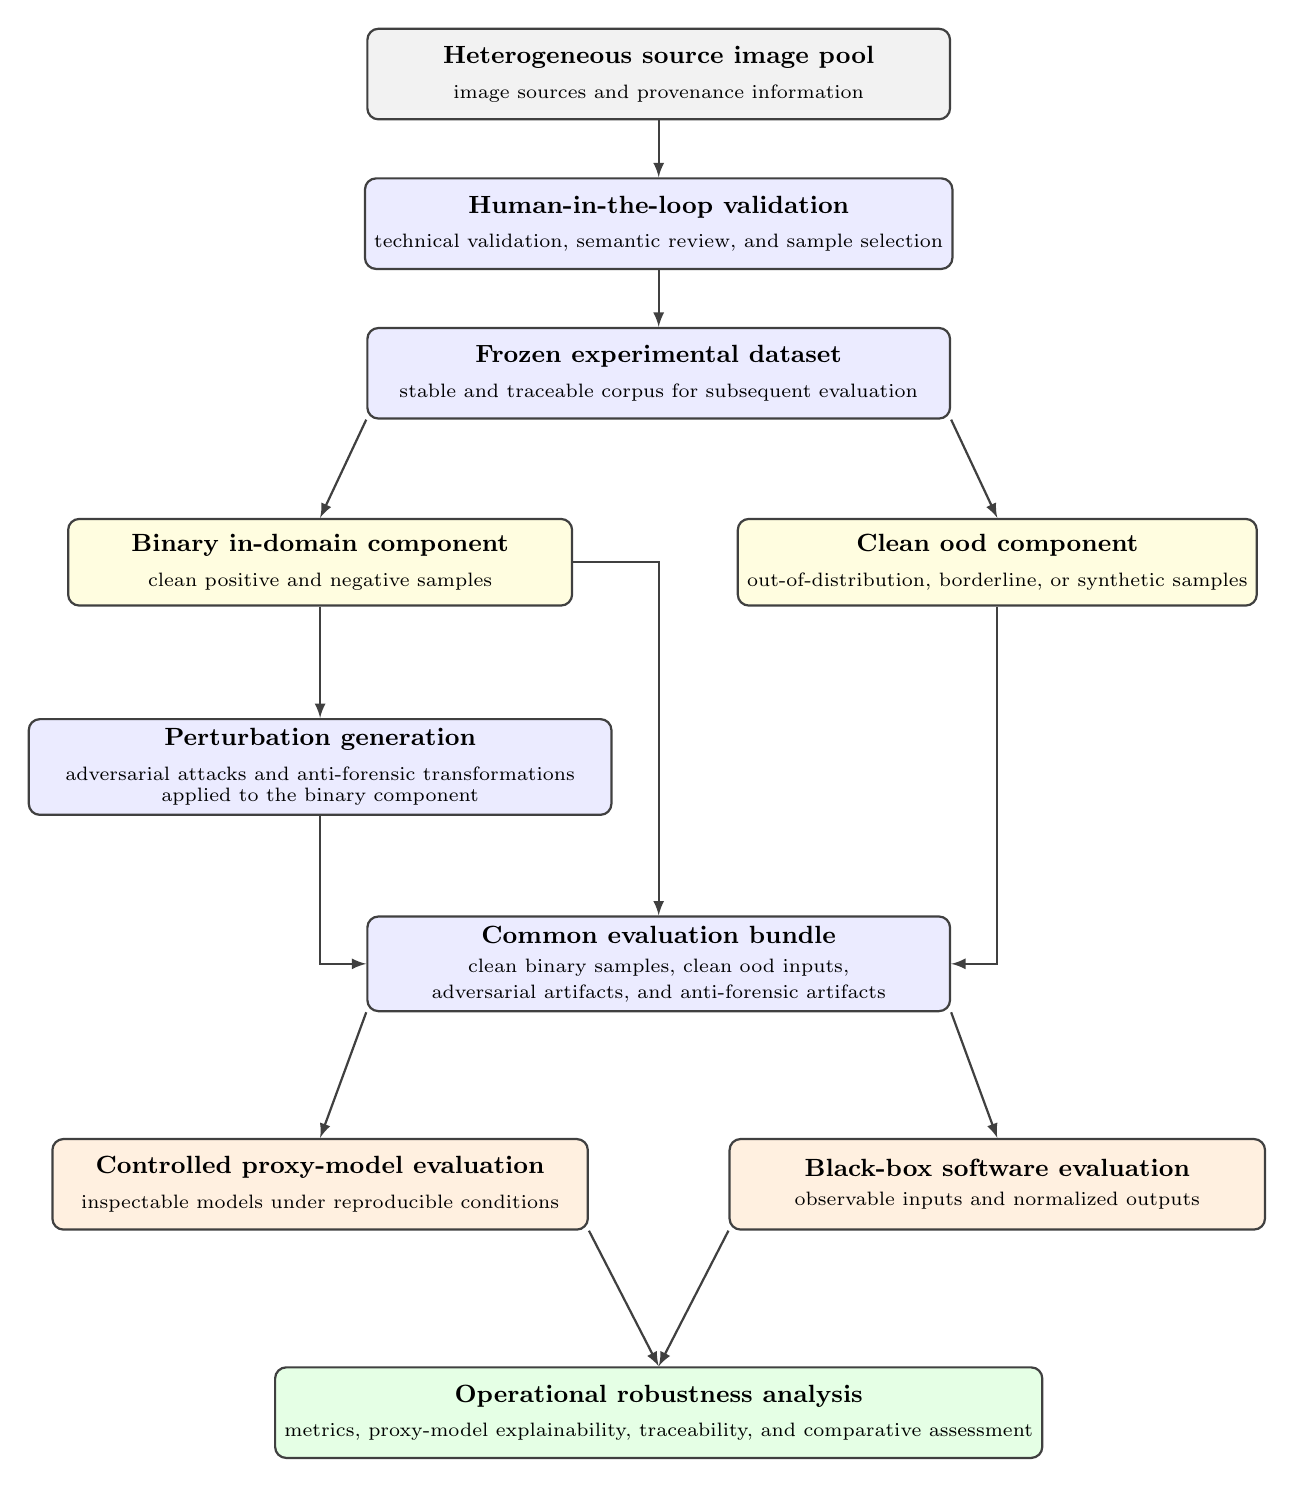
\begin{tikzpicture}[
>=latex,
font=\small,
block/.style={
rectangle,
rounded corners,
draw=black!75,
thick,
align=center,
minimum height=1.15cm,
minimum width=7.4cm,
fill=gray!10
},
process/.style={
rectangle,
rounded corners,
draw=black!75,
thick,
align=center,
minimum height=1.15cm,
minimum width=7.4cm,
fill=blue!8
},
subset/.style={
rectangle,
rounded corners,
draw=black!75,
thick,
align=center,
minimum height=1.10cm,
minimum width=6.4cm,
fill=yellow!12
},
eval/.style={
rectangle,
rounded corners,
draw=black!75,
thick,
align=center,
minimum height=1.15cm,
minimum width=6.8cm,
fill=orange!12
},
output/.style={
rectangle,
rounded corners,
draw=black!75,
thick,
align=center,
minimum height=1.15cm,
minimum width=8.0cm,
fill=green!10
},
arrow/.style={
->,
thick,
draw=black!75
}
]

% -------------------------------------------------------------------------
% Dataset construction
% -------------------------------------------------------------------------
\node[block] (sources) at (0,0)
{\shortstack{
\textbf{Heterogeneous source image pool}\\[1mm]
\scriptsize image sources and provenance information
}};

\node[process] (review) at (0,-1.9)
{\shortstack{
\textbf{Human-in-the-loop validation}\\[1mm]
\scriptsize technical validation, semantic review, and sample selection
}};

\node[process] (dataset) at (0,-3.8)
{\shortstack{
\textbf{Frozen experimental dataset}\\[1mm]
\scriptsize stable and traceable corpus for subsequent evaluation
}};

% -------------------------------------------------------------------------
% Evaluation branches
% -------------------------------------------------------------------------
\node[subset] (binary) at (-4.3,-6.2)
{\shortstack{
\textbf{Binary in-domain component}\\[1mm]
\scriptsize clean positive and negative samples
}};

\node[subset] (ood) at (4.3,-6.2)
{\shortstack{
\textbf{Clean \gls{ood} component}\\[1mm]
\scriptsize out-of-distribution, borderline, or synthetic samples
}};

% -------------------------------------------------------------------------
% Perturbation generation
% -------------------------------------------------------------------------
\node[process] (perturb) at (-4.3,-8.8)
{\shortstack{
\textbf{Perturbation generation}\\[1mm]
\scriptsize adversarial attacks and anti-forensic transformations\\
\scriptsize applied to the binary component
}};

% -------------------------------------------------------------------------
% Common evaluation bundle
% -------------------------------------------------------------------------
\node[process] (bundle) at (0,-11.3)
{\shortstack{
\textbf{Common evaluation bundle}\\[1mm]
\scriptsize clean binary samples, clean \gls{ood} inputs,\\
\scriptsize adversarial artifacts, and anti-forensic artifacts
}};

% -------------------------------------------------------------------------
% Complementary evaluation levels
% -------------------------------------------------------------------------
\node[eval] (proxy) at (-4.3,-14.1)
{\shortstack{
\textbf{Controlled proxy-model evaluation}\\[1mm]
\scriptsize inspectable models under reproducible conditions
}};

\node[eval] (tools) at (4.3,-14.1)
{\shortstack{
\textbf{Black-box software evaluation}\\[1mm]
\scriptsize observable inputs and normalized outputs
}};

% -------------------------------------------------------------------------
% Analysis layer
% -------------------------------------------------------------------------
\node[output] (analysis) at (0,-17.0)
{\shortstack{
\textbf{Operational robustness analysis}\\[1mm]
\scriptsize metrics, proxy-model explainability, traceability, and comparative assessment
}};

% -------------------------------------------------------------------------
% Arrows
% -------------------------------------------------------------------------
\draw[arrow] (sources) -- (review);
\draw[arrow] (review) -- (dataset);

\draw[arrow] (dataset.south west) -- (binary.north);
\draw[arrow] (dataset.south east) -- (ood.north);

\draw[arrow] (binary.south) -- (perturb.north);

% Direct path for the unmodified binary samples.
%\draw[arrow] (binary.west) -- ++(-1.0,0) |- (bundle.west);
\draw[arrow] (binary.east) -- ++(1.0,0) -| (bundle.north);
% Derived adversarial and anti-forensic artifacts.
\draw[arrow] (perturb.south) |- (bundle.west);

% Separate clean OOD branch.
\draw[arrow] (ood.south) |- (bundle.east);

\draw[arrow] (bundle.south west) -- (proxy.north);
\draw[arrow] (bundle.south east) -- (tools.north);

\draw[arrow] (proxy.south east) -- (analysis.north);
\draw[arrow] (tools.south west) -- (analysis.north);

\end{tikzpicture}%
}
\caption[FAIRLab experimental protocol]{FAIRLab experimental protocol. The
frozen corpus is divided into a binary in-domain component and a separate clean
\gls{ood} branch. Perturbations are applied only to the binary component, and
the resulting common bundle is evaluated through complementary proxy-model and
black-box software analyses}
\label{fig:methodology-fairlab-overview}
\end{figure}

% ─────────────────────────────────────────────────────────────────────────────
\section{Research Design and Experimental Assumptions}
\label{sec:methodology-research-design}
% ─────────────────────────────────────────────────────────────────────────────

The experimental design adopts forensic visual triage as its reference
scenario, in which automated classification supports the preliminary
identification and prioritization of potentially relevant images. The case
study defines a controlled firearm-related classification task rather than
attempting to cover the entire domain of weapon detection. This restricted
scope provides a clear target category while retaining sufficient visual
variability for robustness assessment. The adopted designations are operational
categories established for the experiment and must not be interpreted as legal
qualifications or universal semantic classes.

The binary task distinguishes between \texttt{weapon}, defined as the positive
class, and \texttt{non\_weapon}, defined as the in-domain negative class. A
separate \gls{ood} branch is reserved for distributional evaluation and is not
modeled as a third supervised class. The assignment criteria were formalized
before dataset freezing and govern human-in-the-loop validation, sample
selection, and the documentation of inclusion and exclusion decisions.
Table~\ref{tab:methodology-operational-classes} summarizes these operational
definitions.

\begin{table}[H]
\centering
\caption{Operational definitions adopted in the experimental protocol}
\label{tab:methodology-operational-classes}
\footnotesize
\renewcommand{\arraystretch}{1.05}
\begin{tabularx}{\textwidth}{@{}L{3.0cm}L{3.6cm}X@{}}
\toprule
\textbf{Designation} &
\textbf{Role in the protocol} &
\textbf{Operational assignment criterion} \\
\midrule

\texttt{weapon}
&
Positive class of the binary task
&
Images containing clearly recognizable and realistic firearm-related visual
content. Representative examples include pistols, rifles, submachine guns, and
shotguns. The target object must be sufficiently visible and reliably
attributable to the experimental category. Marginal, strongly occluded,
excessively ambiguous, synthetic, toy-like, replica-like, or airsoft-like
objects are excluded from this class. \\

\texttt{non\_weapon}
&
In-domain negative class of the binary task
&
Realistic, usable, and visually interpretable images that do not contain an
object belonging to the experimental target category. Examples may include
people, environments, vehicles, ordinary objects, and indoor or outdoor scenes.
Borderline, synthetic, or anomalous content is excluded. Images containing
knives, swords, replicas, airsoft weapons, toy weapons, videogame weapons, or
rendered weapon-like objects are also excluded because they may introduce
semantic ambiguity. \\

\gls{ood}
&
Separate branch for distributional evaluation
&
Borderline, anomalous, or non-representative images that do not constitute clean
positive or negative samples. Examples include knives, swords, replicas, toys,
airsoft weapons, videogame weapons, \gls{cgi} content, synthetic images,
generated images, tanks, missiles, explosions, and war scenes. The branch may
also include source images that are strongly degraded, unusual, or semantically
ambiguous. These inputs are retained without experimental manipulation and are
not equivalent to the adversarial or anti-forensic artifacts generated in later
stages. Such content may be contextually related to weapons or violence without
constituting a valid sample for the binary task. \\

\texttt{exclude}
&
Review-only exclusion designation
&
Images that are corrupted, unreadable, unusable, non-interpretable, or
semantically irrelevant to the experimental protocol. This designation is used
during human review to document the removal of unsuitable samples. Excluded
images do not contribute to the frozen dataset or to any subsequent evaluation
branch. \\

\bottomrule
\end{tabularx}
\end{table}

Figure~\ref{fig:methodology-class-examples} presents representative examples of
the two binary classes and the separate \gls{ood} branch. The examples are
illustrative and do not exhaust the internal variability of the corresponding
groups.

\begin{figure}[H]
\centering

\begin{minipage}[t]{0.31\textwidth}
\centering
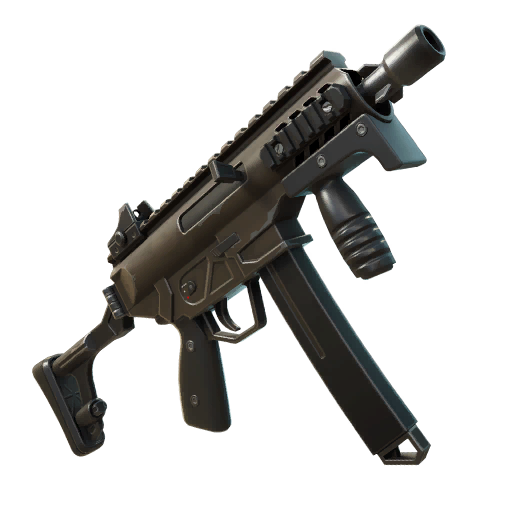
\includegraphics[
width=\textwidth,
height=4.0cm,
keepaspectratio
]{images/Arma}
\vspace{1mm}

\textbf{\texttt{weapon}}\\
\footnotesize
Recognizable firearm-related content consistent with the binary target class
\end{minipage}
\hfill
\begin{minipage}[t]{0.31\textwidth}
\centering

\includegraphics[
width=\textwidth,
height=4.0cm,
keepaspectratio
]{images/Non_Arma}
\vspace{1mm}

\textbf{\texttt{non\_weapon}}\\
\footnotesize
Realistic negative content containing no object from the target category
\end{minipage}
\hfill
\begin{minipage}[t]{0.31\textwidth}
\centering

\includegraphics[
width=\textwidth,
height=4.0cm,
keepaspectratio
]{images/ood}
\vspace{1mm}

\textbf{\gls{ood}}\\
\footnotesize
Borderline or distributionally different content kept outside the binary task
\end{minipage}

\caption[Representative operational class and OOD examples]{Representative
examples of the binary operational classes and the separate \gls{ood} branch
adopted during human-in-the-loop review}
\label{fig:methodology-class-examples}
\end{figure}

The \texttt{exclude} designation is used exclusively as a quality-control
disposition during human review and does not constitute an additional
analytical branch. Likewise, the \gls{ood} branch is not a homogeneous semantic
class or a subclass of \texttt{non\_weapon}. It contains borderline,
anomalous, degraded, synthetic, or otherwise distributionally different inputs
that do not constitute clean instances of either binary class. Since
classifiers may produce high-confidence predictions outside their training
distribution \cite{hendrycks2017baseline,fort2021exploring}, these inputs must
be assessed separately from ordinary binary errors. Their exclusion from model
training and perturbation generation is formalized in
Section~\ref{sec:methodology-split-generation}.

These operational definitions provide the semantic basis for the dataset
construction, review-documentation, and freezing procedures described in
Sections~\ref{sec:methodology-dataset-construction},
\ref{sec:methodology-review-manifest}, and
\ref{sec:methodology-human-review}. They ensure that final assignments are
derived from explicit and traceable review criteria rather than inherited
directly from source labels, filenames, or directory structures.

% ─────────────────────────────────────────────────────────────────────────────
\section{Dataset Construction and Source Consolidation}
\label{sec:methodology-dataset-construction}
% ─────────────────────────────────────────────────────────────────────────────

Dataset construction separates source collection, technical validation,
semantic review, and final dataset freezing. This distinction is
methodologically necessary because the technical validity of an image file
does not establish its semantic suitability for the forensic classification
task.

The process begins with the consolidation of heterogeneous image sources into
a candidate pool. The objective is not to create a visually homogeneous
collection, but to capture part of the variability encountered in contemporary
digital investigations. Depending on the investigated domain and data
availability, the candidate pool may include public datasets, specialized
repositories, open-web content, \gls{osint}-oriented collections, and material
obtained from less structured or non-indexed online environments.

The composition and relative contribution of these sources may vary, but the
provenance of each candidate sample must remain identifiable throughout the
preparation and review process.
Table~\ref{tab:methodology-raw-sources} summarizes the methodological roles of
the source categories considered in the protocol.

\begin{table}[H]
\centering
\caption{Methodological roles of the image-source categories}
\label{tab:methodology-raw-sources}
\begin{tabularx}{\textwidth}{@{}L{4.2cm}X@{}}
\toprule
\textbf{Source category} &
\textbf{Methodological role} \\
\midrule

Public datasets
&
Provide structured and reproducible collections that can support the initial
construction of the candidate pool. Their original labels are retained as
source information and are not automatically inherited as experimentally
validated reference assignments. \\

Specialized repositories
&
Provide domain-specific images that can improve the representation of candidate
content related to the target visual category. Samples obtained from these
sources remain subject to the same validation and assignment criteria applied
to the rest of the candidate pool. \\

Open-web collections
&
Introduce greater variability in image quality, composition, context, and
acquisition conditions. They reduce dependence on curated benchmark
distributions. \\

\gls{osint}-oriented sources
&
Represent less structured content obtained from social, multimedia, or other
openly accessible investigative sources. They contribute operationally relevant
variability. \\

Non-indexed or unconventional online sources
&
Provide heterogeneous material that may differ from conventional public
datasets in content, quality, context, or distribution. Their inclusion supports
the evaluation of less standardized acquisition contexts. \\

\bottomrule
\end{tabularx}
\end{table}

After source consolidation, candidate images undergo technical validation
before any semantic assignment is made. The validation process verifies that
each file can be processed reliably and may include readability, structural
validity, dimensional suitability, duplicate detection, and stable sample
identification. The resulting records must preserve sufficient information to
associate each retained sample with its provenance, technical-validation
outcome, and integrity information.

Source location, directory structure, filename, and pre-existing annotations
may be retained as contextual or audit information, but they must not be
treated as definitive reference assignments. Final semantic membership must
instead be determined through the operational criteria defined in
Section~\ref{sec:methodology-research-design}. This separation limits the
propagation of source-specific assumptions and labeling errors into the frozen
experimental dataset.

The relative size of the original source collections must also be considered
during sample selection. A large or highly asymmetric source must not
automatically dominate the final corpus. Composition decisions should instead
reflect the experimental objectives, the required class structure, and the
need to preserve meaningful source diversity.

Following technical validation, the candidate pool is submitted to the
documented semantic-review process described in
Sections~\ref{sec:methodology-review-manifest} and
\ref{sec:methodology-human-review}. Figure~\ref{fig:methodology-dataset-source-consolidation}
summarizes the transition from heterogeneous sources to the frozen
experimental dataset.

\begin{figure}[H]
\centering
\resizebox{0.62\textwidth}{!}{%
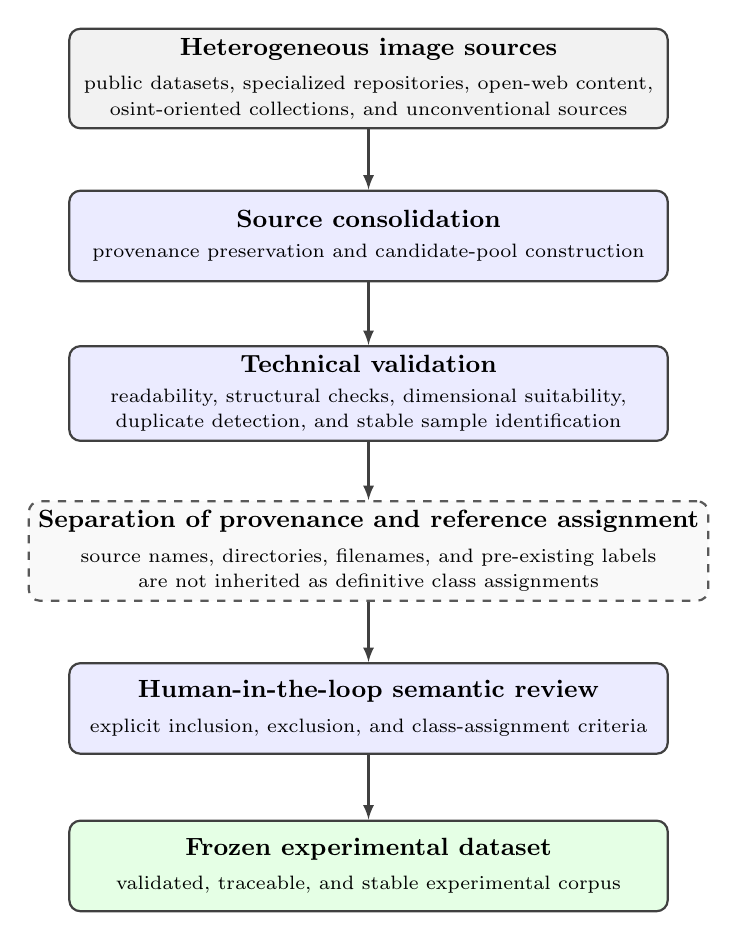
\begin{tikzpicture}[
>=latex,
font=\small,
block/.style={
rectangle,
rounded corners,
draw=black!75,
thick,
align=center,
minimum height=1.15cm,
minimum width=7.6cm,
fill=gray!10
},
process/.style={
rectangle,
rounded corners,
draw=black!75,
thick,
align=center,
minimum height=1.15cm,
minimum width=7.6cm,
fill=blue!8
},
note/.style={
rectangle,
rounded corners,
draw=black!65,
dashed,
thick,
align=center,
minimum height=1.05cm,
minimum width=7.6cm,
fill=gray!5
},
final/.style={
rectangle,
rounded corners,
draw=black!75,
thick,
align=center,
minimum height=1.15cm,
minimum width=7.6cm,
fill=green!10
},
arrow/.style={
->,
thick,
draw=black!75
}
]

\node[block] (sources) at (0,0)
{\shortstack{
\textbf{Heterogeneous image sources}\\[1mm]
\scriptsize public datasets, specialized repositories, open-web content,\\
\scriptsize \gls{osint}-oriented collections, and unconventional sources
}};

\node[process] (consolidation) at (0,-2.0)
{\shortstack{
\textbf{Source consolidation}\\[1mm]
\scriptsize provenance preservation and candidate-pool construction
}};

\node[process] (validation) at (0,-4.0)
{\shortstack{
\textbf{Technical validation}\\[1mm]
\scriptsize readability, structural checks, dimensional suitability,\\
\scriptsize duplicate detection, and stable sample identification
}};

\node[note] (separation) at (0,-6.0)
{\shortstack{
\textbf{Separation of provenance and reference assignment}\\[1mm]
\scriptsize source names, directories, filenames, and pre-existing labels\\
\scriptsize are not inherited as definitive class assignments
}};

\node[process] (review) at (0,-8.0)
{\shortstack{
\textbf{Human-in-the-loop semantic review}\\[1mm]
\scriptsize explicit inclusion, exclusion, and class-assignment criteria
}};

\node[final] (frozen) at (0,-10.0)
{\shortstack{
\textbf{Frozen experimental dataset}\\[1mm]
\scriptsize validated, traceable, and stable experimental corpus
}};

\draw[arrow] (sources) -- (consolidation);
\draw[arrow] (consolidation) -- (validation);
\draw[arrow] (validation) -- (separation);
\draw[arrow] (separation) -- (review);
\draw[arrow] (review) -- (frozen);

\end{tikzpicture}%
}
\caption[Dataset source consolidation]{Dataset source consolidation.
Heterogeneous sources are combined into a traceable candidate pool, subjected
to technical validation, and reviewed according to explicit semantic criteria.
Final class assignments are not inherited from source directories, filenames,
or pre-existing annotations}
\label{fig:methodology-dataset-source-consolidation}
\end{figure}

% ─────────────────────────────────────────────────────────────────────────────
\section{Review Documentation and Semantic Decision Records}
\label{sec:methodology-review-manifest}
% ─────────────────────────────────────────────────────────────────────────────

Following technical validation, each candidate sample is associated with a
structured review record that connects its technical preparation to the
subsequent human-in-the-loop semantic assessment. The record must preserve two
distinct categories of information: sample identity, provenance, technical
validity, and integrity information; and the semantic decision produced during
manual review, including review status, operational assignment, exclusion
disposition, explanatory notes, and any information required to document
ambiguous or \gls{ood} cases.

Regardless of its technical representation, the review record must maintain a
stable association among the candidate sample, its provenance, the documented
semantic decision, and any experimental artifact subsequently derived from it.
This association enables the decision process and the transition from the
candidate pool to the frozen experimental dataset to be reconstructed.

Labels inherited from source material or generated through automated
preprocessing may be retained as contextual information, but they must not
replace the explicit semantic judgment produced during human-in-the-loop
review. Final operational assignments are determined exclusively according to
the criteria defined in
Section~\ref{sec:methodology-research-design}.

The separation between technical-validation information and semantic decision
records preserves the distinction between file suitability and relevance to
the experimental task. The resulting documentation supports the consistent
application of the assignment criteria, preserves the rationale for inclusion,
exclusion, and class-assignment decisions, and provides the traceability
required for the review and dataset-freezing procedure described in
Section~\ref{sec:methodology-human-review}.

% ─────────────────────────────────────────────────────────────────────────────
\section{Human-in-the-Loop Review and Final Dataset Freezing}
\label{sec:methodology-human-review}
% ─────────────────────────────────────────────────────────────────────────────

The technically validated candidate pool is subjected to a documented
\textit{human-in-the-loop} review to determine the semantic suitability of each
sample and assign the corresponding operational designation. The criteria
defined in Section~\ref{sec:methodology-research-design} must be applied
consistently and independently of source directories, filenames, inherited
annotations, or automated pre-labels.

The review follows a conservative decision rule. Samples are included in the
binary task only when they can be assigned to either \texttt{weapon} or
\texttt{non\_weapon} with sufficient semantic clarity. Borderline, anomalous,
synthetic, replica-like, degraded, or otherwise distributionally different
content is retained within the separate \gls{ood} branch rather than being
forced into either binary class. Unusable or semantically irrelevant samples
are assigned to the review-only \texttt{exclude} disposition.

These assignments are operational designations defined for the experimental
protocol and must not be interpreted as definitive legal, material, or
evidentiary determinations regarding the depicted content. In particular,
assignment to the \gls{ood} branch represents a methodological decision for
cases that do not constitute clear instances of either binary class.

Each review decision must remain reconstructable through the semantic decision
records defined in Section~\ref{sec:methodology-review-manifest}. These records
preserve the association among the reviewed sample, its provenance, the
assigned disposition, any explanatory notes, and the experimental artifacts
subsequently derived from it.

After all candidate samples have been reviewed, the selected corpus is frozen.
Dataset freezing establishes a stable reference corpus whose composition
remains unchanged throughout the subsequent evaluation phases. Any correction
or modification introduced after freezing must be explicitly documented and
treated as a new version of the experimental dataset.

The frozen dataset provides the common source corpus for the controlled
proxy-model evaluation and the black-box evaluation of the selected
\gls{ai}-based software systems. Its subsequent separation into the binary
evaluation subset and the clean \gls{ood} branch is defined in
Section~\ref{sec:methodology-split-generation}.

The number of reviewers and the review workflow may vary across
implementations. When the protocol is conducted by a single reviewer, the
absence of inter-annotator agreement must be acknowledged as a limitation.
Explicit assignment criteria, structured decision records, and dataset
freezing support procedural auditability and reproducibility, but do not
eliminate the subjectivity inherent in semantic assessment. Dataset freezing
therefore acts as a methodological control that distinguishes changes in
systems, perturbations, and metrics from undocumented changes in the evaluated
corpus.











% ─────────────────────────────────────────────────────────────────────────────
\section{Data Partitioning and OOD Evaluation Strategy}
\label{sec:methodology-split-generation}
% ─────────────────────────────────────────────────────────────────────────────

After dataset freezing, the experimental corpus is divided into two distinct
branches: an in-domain binary subset and a separate \gls{ood} evaluation set.
This separation reflects the different methodological purposes of the two
components. The binary subset supports model training, clean evaluation, and
robustness testing, whereas the \gls{ood} set is used to examine system behavior
on borderline, semantically atypical, or distributionally different inputs.

The binary subset is organized into mutually exclusive experimental
partitions, hereafter referred to as folds. The number and size of these folds
depend on the available dataset, the class distribution, and the requirements
of the experimental design. The methodology therefore does not prescribe a
fixed number of folds or a specific directory organization.

Regardless of the adopted configuration, the partitioning procedure must
satisfy four requirements. First, each sample must belong to only one fold.
Second, the class distribution should remain sufficiently consistent across
folds whenever the dataset permits stratified partitioning. Third, sample
identity and provenance must remain traceable. Fourth, the allocation procedure
must be deterministic or otherwise documented in sufficient detail to allow the
partitions to be regenerated.

Within this protocol, folds are not introduced primarily as a conventional
cross-validation mechanism for hyperparameter selection or general performance
estimation. Instead, they define controlled experimental holdout units. For
each target fold, the proxy classification model is trained on the remaining
folds and evaluated on the held-out samples.

This fold-aware organization prevents overlap between the samples used for
model fitting and those used for clean and robustness evaluation. It also
preserves a consistent association between each held-out sample, the
corresponding proxy-model checkpoint, and any model-dependent adversarial
artifact generated from that sample. Model-agnostic anti-forensic
transformations remain associated with the originating sample and its assigned
fold but do not depend on a specific model checkpoint.

The specific number of folds is an implementation choice rather than a general
methodological requirement. A study may adopt a different number of partitions
provided that the resulting organization preserves separation, traceability,
and sufficient representation of the relevant classes.

The \gls{ood} samples are kept outside the binary folds. They are not used to
train the proxy classification models and are not treated as a third supervised
class. They are also excluded from the generation of adversarial and
anti-forensic variants because they address a different experimental question.

More specifically, the \gls{ood} evaluation examines how an automated system
assigns content that should not be treated as an ordinary
\texttt{weapon} or \texttt{non\_weapon} sample relative to the known
operational classes. The branch is kept clean in the methodological sense that
no experimental adversarial perturbation or anti-forensic transformation is
applied to its samples. This separation prevents distributional mismatch from
being conflated with deliberate or incidental input manipulation.

The partitioning procedure must produce structured records that associate each
sample with its evaluation branch and, when applicable, its fold. These records
should preserve sample identity, provenance, operational assignment, integrity
information, and the relationship between the original image and any derived
experimental artifact. The methodology does not impose a specific file format,
hashing algorithm, or storage technology.

Figure~\ref{fig:methodology-split-to-proxy-training} summarizes the general
partitioning strategy. The frozen dataset is separated into a binary in-domain
branch and a clean \gls{ood} branch. The binary samples are organized into
mutually exclusive folds used for fold-aware training and held-out evaluation,
whereas the \gls{ood} samples remain outside the training and perturbation
generation processes.

\begin{figure}[H]
\centering
\resizebox{0.94\textwidth}{!}{%
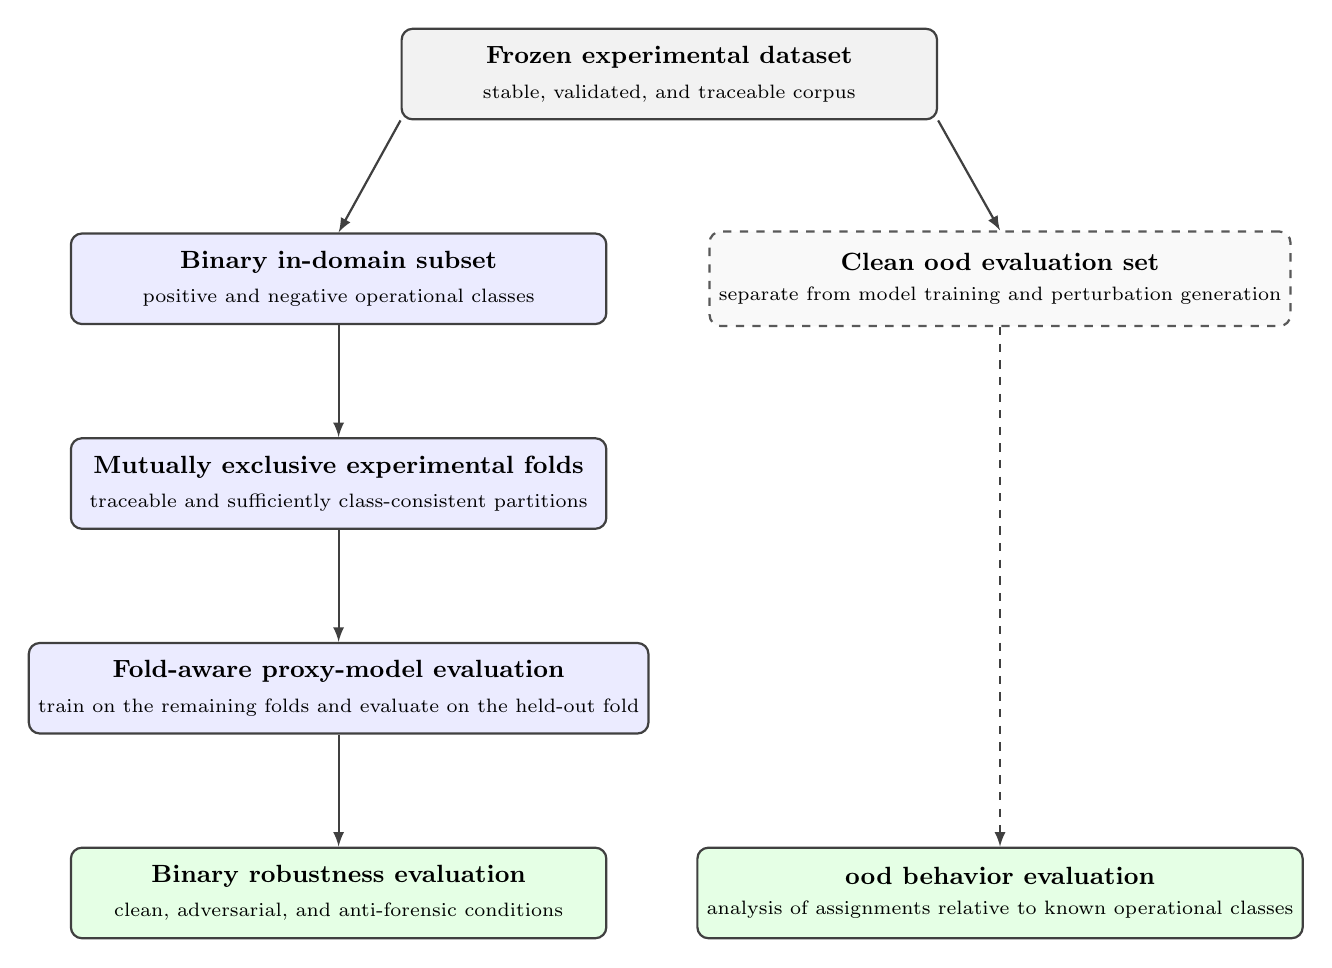
\begin{tikzpicture}[
>=latex,
font=\small,
block/.style={
rectangle,
rounded corners,
draw=black!75,
thick,
align=center,
minimum height=1.15cm,
minimum width=6.8cm,
fill=gray!10
},
process/.style={
rectangle,
rounded corners,
draw=black!75,
thick,
align=center,
minimum height=1.15cm,
minimum width=6.8cm,
fill=blue!8
},
output/.style={
rectangle,
rounded corners,
draw=black!75,
thick,
align=center,
minimum height=1.15cm,
minimum width=6.8cm,
fill=green!10
},
note/.style={
rectangle,
rounded corners,
draw=black!65,
dashed,
thick,
align=center,
minimum height=1.20cm,
minimum width=6.8cm,
fill=gray!5
},
arrow/.style={
->,
thick,
draw=black!75
},
dashedarrow/.style={
->,
thick,
dashed,
draw=black!75
}
]

\node[block] (frozen) at (0,0)
{\shortstack{
\textbf{Frozen experimental dataset}\\[1mm]
\scriptsize stable, validated, and traceable corpus
}};

\node[process] (binary) at (-4.2,-2.6)
{\shortstack{
\textbf{Binary in-domain subset}\\[1mm]
\scriptsize positive and negative operational classes
}};

\node[note] (ood) at (4.2,-2.6)
{\shortstack{
\textbf{Clean \gls{ood} evaluation set}\\[1mm]
\scriptsize separate from model training and perturbation generation
}};

\node[process] (folds) at (-4.2,-5.2)
{\shortstack{
\textbf{Mutually exclusive experimental folds}\\[1mm]
\scriptsize traceable and sufficiently class-consistent partitions
}};

\node[process] (training) at (-4.2,-7.8)
{\shortstack{
\textbf{Fold-aware proxy-model evaluation}\\[1mm]
\scriptsize train on the remaining folds and evaluate on the held-out fold
}};

\node[output] (binaryevaluation) at (-4.2,-10.4)
{\shortstack{
\textbf{Binary robustness evaluation}\\[1mm]
\scriptsize clean, adversarial, and anti-forensic conditions
}};

\node[output] (oodevaluation) at (4.2,-10.4)
{\shortstack{
\textbf{\gls{ood} behavior evaluation}\\[1mm]
\scriptsize analysis of assignments relative to known operational classes
}};

\draw[arrow] (frozen.south west) -- (binary.north);
\draw[arrow] (frozen.south east) -- (ood.north);

\draw[arrow] (binary) -- (folds);
\draw[arrow] (folds) -- (training);
\draw[arrow] (training) -- (binaryevaluation);

\draw[dashedarrow] (ood) -- (oodevaluation);

\end{tikzpicture}%
}
\caption[Data partitioning and OOD evaluation strategy]{Data partitioning and
OOD evaluation strategy. The binary subset is organized into mutually exclusive
folds for fold-aware training and held-out evaluation, while the clean
\gls{ood} branch remains outside model training and perturbation generation}
\label{fig:methodology-split-to-proxy-training}
\end{figure}


% ─────────────────────────────────────────────────────────────────────────────
\section{Proxy-Model Evaluation Framework}
\label{sec:methodology-models-classification}
% ─────────────────────────────────────────────────────────────────────────────

The controlled component of the methodology relies on a set of fully
inspectable classification models, hereafter referred to as
\textit{proxy classification models}. In this thesis, proxy models are fully
inspectable experimental reference models used to study controlled
classification behavior, robustness degradation, transferability, confidence
patterns, and error direction under reproducible conditions.

Proxy classification models are not replicas, functionally equivalent
substitutes, reverse-engineered reconstructions, or architectural reproductions
of the selected black-box software systems. Their role is to provide an
experimental environment in which model architecture, training procedure,
class mapping, checkpoints, and decision behavior can be inspected and
controlled.

The proxy-model framework supports three methodological objectives. First, it
provides a transparent reference for measuring classification performance and
robustness degradation. Second, it enables the generation of model-dependent
adversarial examples under explicitly defined access assumptions, including
white-box and score-based conditions. Third, it supports the analysis of whether
perturbations generated against one controlled model transfer to other proxy
architectures or to selected black-box software systems.

The proxy models implement the binary classification task defined in
Section~\ref{sec:methodology-research-design}. The two operational classes are
\texttt{non\_weapon} and \texttt{weapon}. Their numerical encoding is an
implementation choice and does not constitute a methodological requirement,
provided that the mapping remains explicit and consistent throughout training,
evaluation, and metric computation.

The \gls{ood} branch is excluded from proxy-model training and is not treated as
a third supervised class. It remains reserved for the separate evaluation of
system behavior on borderline, semantically atypical, or distributionally
different content, as described in
Section~\ref{sec:methodology-split-generation}. This separation prevents binary
robustness from being conflated with system behavior on samples outside the
operational distribution.

The methodology does not prescribe specific model architectures. Instead, the
controlled evaluation should include models with complementary algorithmic
characteristics. Depending on the experimental context, these may include
conventional convolutional architectures, efficiency-oriented architectures,
and models based on large-scale pretrained visual representations.

The selected models should be sufficiently documented to support reproducible
training and evaluation. Relevant information includes the architecture,
initialization strategy, preprocessing procedure, class mapping, optimization
method, training configuration, and identity of the resulting checkpoints. The
concrete architectures and configurations adopted in this thesis are reported
in Chapter~\ref{chap:implementation}.

Proxy-model training follows the fold-aware strategy introduced in
Section~\ref{sec:methodology-split-generation}. For each target fold, the
corresponding model instance is trained exclusively on the remaining folds and
evaluated on the held-out samples. This organization preserves the separation
between model fitting and experimental evaluation.

The same separation must be maintained during model-dependent perturbation
generation. An adversarial artifact associated with a held-out sample must be
generated using a model checkpoint that was not trained on that sample. This
requirement reduces the risk of information leakage and preserves the validity
of the subsequent robustness analysis.

Training conditions should remain consistent across folds for a given model
configuration. This consistency ensures that observed differences among folds
are attributable primarily to the evaluated samples rather than to unintended
changes in the optimization procedure. Any variation in architecture,
preprocessing, initialization, or training parameters must be explicitly
documented.

For model-dependent adversarial attacks, the protocol designates one controlled
model as the \textit{primary proxy target}. This model acts as the source system
against which adversarial examples are generated under the access assumptions
required by each attack. White-box attacks may use gradients, decision
boundaries, or other internal model information, whereas score-based attacks
rely on observable model scores without requiring direct access to gradients.
The choice of the primary proxy target is an implementation decision and does
not imply that the selected architecture is universally more accurate, more
representative, or more robust than the alternatives.

The use of a primary proxy target limits unnecessary multiplication of
experimental variants. Rather than optimizing every model-dependent attack
separately against every architecture, the protocol generates a coherent
adversarial test set against one documented source model. The resulting
artifacts are then evaluated on the remaining proxy models to examine
cross-model transferability.

For model-dependent adversarial artifacts, this procedure distinguishes three
evaluation conditions:

\begin{enumerate}
\item \textit{direct source-model evaluation}, in which adversarial
artifacts are assessed against the proxy-model checkpoint used to generate
them under the corresponding access assumptions;

\item \textit{cross-model transfer evaluation}, in which the same artifacts
are assessed against different proxy architectures;

\item \textit{black-box transfer evaluation}, in which the same artifacts
are submitted to the selected black-box software systems.
\end{enumerate}

Anti-forensic transformations follow a different rationale. They are applied
directly to the image according to controlled transformation rules and are not
optimized against the gradients, scores, or decision boundary of a specific
model. Their evaluation therefore concerns the stability of classification
behavior under operationally relevant image modifications rather than the
success of an optimization procedure against a designated source model.

Model-agnostic adversarial-style conditions must also be distinguished from
transfer attacks. Because they are generated without reference to a source
model, their evaluation across different proxy models and black-box software
systems measures response stability under a shared manipulated condition rather
than adversarial transferability.

The distinction among white-box, score-based, and model-agnostic conditions is
methodologically important. Model-dependent adversarial attacks evaluate
vulnerability under explicit access assumptions. Model-agnostic adversarial-
style conditions and anti-forensic transformations instead assess whether
controlled changes to image encoding, dimensions, visual quality, or appearance
alter the observable classification outcome.

Finally, the proxy-model framework must remain separate from the operational
evaluation of the selected black-box software systems. Proxy models are
inspectable and configurable components for which training conditions and model
artifacts are known. The selected software systems are evaluated under
black-box or near-black-box access conditions, without assuming access to their
internal architectures, training data, calibration procedures, or decision
logic.

This separation enables the methodology to combine experimental control with
operational relevance. Proxy models support the controlled analysis of how
documented architectures respond under reproducible conditions, while black-box
evaluation measures the observable behavior of operationally relevant software
systems when exposed to the same clean samples, clean \gls{ood} inputs,
adversarial artifacts, and anti-forensic artifacts.


% ─────────────────────────────────────────────────────────────────────────────
\section{Perturbation Selection Rationale and Operational Relevance}
\label{sec:methodology-perturbation-selection-rationale}
% ─────────────────────────────────────────────────────────────────────────────

The perturbation framework is designed to evaluate classification behavior
under controlled input modifications that differ in access assumptions,
computational cost, perceptual impact, and operational plausibility. The
selection process is therefore not based exclusively on the theoretical
strength of individual attacks. It also considers whether the resulting
experimental conditions are reproducible and relevant to realistic
\gls{df} workflows.

In forensic visual triage, automated systems may be required to process large
image collections within operational time constraints. Computational cost is
therefore methodologically relevant. A perturbation that requires extensive
optimization for each image may be useful for controlled vulnerability
analysis, but may be less representative of manipulations that can be applied
rapidly and at scale.

The methodology distinguishes among three broad categories of input
modification:

\begin{enumerate}
\item \textit{model-dependent adversarial attacks}, which are generated
against a designated source model under explicit white-box or score-based
access assumptions;

\item \textit{model-agnostic adversarial-style conditions}, which alter the
image according to predefined rules without being optimized against a
specific classifier;

\item \textit{anti-forensic transformations}, which emulate plausible
modifications of the image artifact or its visual representation.
\end{enumerate}

Model-dependent adversarial attacks provide controlled tests of classifier
vulnerability under explicit access assumptions. Depending on the selected
algorithm, they may involve a single gradient computation, an iterative
procedure, an optimization process, a decision-boundary search, or repeated
queries to observable model scores.

These attacks are included primarily to investigate sensitivity, attack
effectiveness, and transferability. They do not necessarily represent the most
probable manipulation in an ordinary forensic scenario. Their operational
relevance instead lies in demonstrating how classification behavior may change
when an actor deliberately exploits information obtained from, or interaction
with, the designated source model.

Model-agnostic adversarial-style conditions do not require access to the
internal properties or observable scores of a specific classifier. They modify
image characteristics according to predefined rules and can therefore be
generated independently of the evaluated systems. Their application across
multiple proxy architectures and black-box software systems supports comparison
under a shared manipulated condition rather than transferability analysis from
a designated source model.

Anti-forensic transformations emulate common or plausible image-processing
operations that may occur deliberately or incidentally before forensic
acquisition or analysis. Relevant transformation families include lossy
re-encoding, resampling, resizing, filtering, tonal modification, and contrast
adjustment.

Such transformations are generally inexpensive and suitable for batch
processing. They are therefore operationally relevant because they may be
applied to large collections without requiring access to the evaluated
classifier. They may also arise from ordinary image-handling processes,
including editing, forwarding, recompression, platform-mediated conversion, or
content normalization.

The perturbation set should provide complementary experimental coverage rather
than several near-duplicate variants of the same manipulation. Selection should
therefore consider the following criteria:

\begin{itemize}
\item diversity of access assumptions;
\item diversity of algorithmic mechanisms;
\item computational feasibility and scalability;
\item reproducibility across experimental runs;
\item preservation or degradation of semantic content;
\item operational plausibility;
\item suitability for cross-system comparison and, where applicable,
transferability analysis;
\item compatibility with the evaluated image formats and software systems.
\end{itemize}

Table~\ref{tab:methodology-attack-cost-operational-relevance} summarizes the
general relationship between perturbation category, computational cost, and
operational relevance.

\begin{table}[H]
\centering
\caption{Perturbation categories, computational cost, and operational relevance}
\label{tab:methodology-attack-cost-operational-relevance}
\begin{tabularx}{\textwidth}{@{}
>{\raggedright\arraybackslash}p{0.25\textwidth}
>{\raggedright\arraybackslash}p{0.18\textwidth}
X
@{}}
\toprule
\textbf{Perturbation category} &
\textbf{Typical cost} &
\textbf{Methodological and operational role} \\
\midrule

Single-step white-box attacks
&
Low to medium
&
Provide efficient baselines for evaluating sensitivity to gradient-informed
input modifications. \\

Iterative or optimization-based white-box attacks
&
Medium to high
&
Support controlled analysis of decision-boundary vulnerability and minimal or
targeted input modifications. \\

Score-based attacks
&
Medium to high
&
Evaluate vulnerability through repeated interaction with observable model
scores without requiring direct access to gradients or internal parameters. \\

Model-agnostic adversarial-style conditions
&
Low to medium
&
Enable source-model-independent testing through predefined changes to image
appearance or statistical characteristics. \\

Lossy re-encoding and resampling
&
Low
&
Represent common modifications caused by editing, forwarding, format
conversion, or platform-mediated processing. \\

Filtering and degradation
&
Low
&
Assess whether the reduction or alteration of discriminative visual details
affects classification behavior. \\

Tonal and chromatic transformations
&
Low
&
Evaluate sensitivity to changes in color, contrast, luminance, or statistical
image properties. \\

\bottomrule
\end{tabularx}
\end{table}

The cost levels reported in
Table~\ref{tab:methodology-attack-cost-operational-relevance} constitute a
qualitative methodological assessment rather than measured execution times.
Actual runtime depends on the algorithm, hardware, software libraries, image
dimensions, degree of parallelization, and implementation choices.

The qualitative distinction is based on the general algorithmic properties of
the perturbations. Direct transformations generally support efficient batch
processing. Single-step white-box attacks require limited model interaction,
whereas score-based, iterative, and optimization-based attacks may require
repeated inference, model queries, or gradient computation.

This distinction enables computational feasibility and operational plausibility
to be considered without introducing timing measurements that were not
collected systematically. The concrete attacks, transformations, parameter
values, and execution configurations adopted in this thesis are reported in
Chapter~\ref{chap:implementation}.

Adversarial and anti-forensic perturbations are generated exclusively from the
binary in-domain subset. The clean \gls{ood} set remains outside this process
because it addresses distributional mismatch rather than robustness to input
manipulation.

Each generated artifact must remain associated with its source image, the
applied perturbation family, the relevant configuration, and the evaluation
condition. For model-dependent adversarial attacks, the record must also
preserve the identity of the source-model checkpoint and the corresponding
access assumption. This association supports reproducibility and ensures that
the same artifacts can be evaluated across the proxy models and the selected
black-box software systems.

Figure~\ref{fig:methodology-perturbation-workflow} summarizes the general
perturbation workflow. The clean binary subset is processed through separate
adversarial and anti-forensic branches. The resulting artifacts are then
integrated into the common evaluation bundle, together with the unmodified
binary samples and the separate clean \gls{ood} inputs.

\begin{figure}[H]
\centering
\resizebox{0.96\textwidth}{!}{%
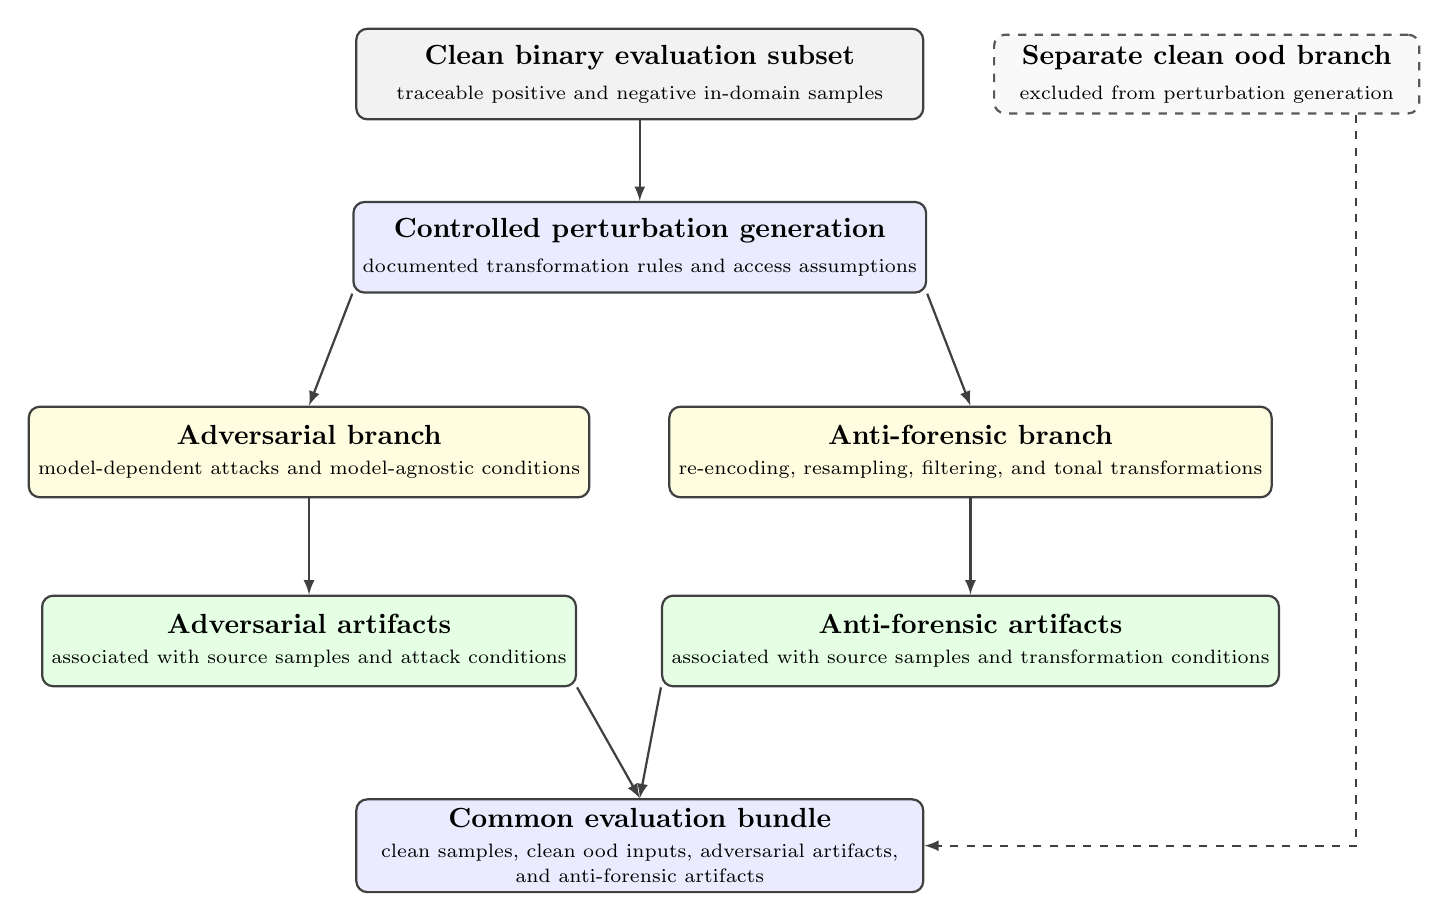
\begin{tikzpicture}[
>=latex,
font=\normalfont,
block/.style={
rectangle,
rounded corners,
draw=black!75,
thick,
align=center,
minimum height=1.15cm,
minimum width=7.2cm,
fill=gray!10
},
process/.style={
rectangle,
rounded corners,
draw=black!75,
thick,
align=center,
minimum height=1.15cm,
minimum width=7.2cm,
fill=blue!8
},
branch/.style={
rectangle,
rounded corners,
draw=black!75,
thick,
align=center,
minimum height=1.15cm,
minimum width=5.8cm,
fill=yellow!12
},
output/.style={
rectangle,
rounded corners,
draw=black!75,
thick,
align=center,
minimum height=1.15cm,
minimum width=5.8cm,
fill=green!10
},
note/.style={
rectangle,
rounded corners,
draw=black!65,
dashed,
thick,
align=center,
minimum height=1.00cm,
minimum width=5.4cm,
fill=gray!5
},
arrow/.style={
->,
thick,
draw=black!75
},
dashedarrow/.style={
->,
thick,
dashed,
draw=black!75
}
]

\node[block] (binary) at (0,0)
{\shortstack{
\textbf{Clean binary evaluation subset}\\[1mm]
\scriptsize traceable positive and negative in-domain samples
}};

\node[process] (generation) at (0,-2.2)
{\shortstack{
\textbf{Controlled perturbation generation}\\[1mm]
\scriptsize documented transformation rules and access assumptions
}};

\node[note] (ood) at (7.2,0)
{\shortstack{
\textbf{Separate clean \gls{ood} branch}\\[1mm]
\scriptsize excluded from perturbation generation
}};

\node[branch] (adversarial) at (-4.2,-4.8)
{\shortstack{
\textbf{Adversarial branch}\\[1mm]
\scriptsize model-dependent attacks and model-agnostic conditions
}};

\node[branch] (antiforensic) at (4.2,-4.8)
{\shortstack{
\textbf{Anti-forensic branch}\\[1mm]
\scriptsize re-encoding, resampling, filtering, and tonal transformations
}};

\node[output] (advartifacts) at (-4.2,-7.2)
{\shortstack{
\textbf{Adversarial artifacts}\\[1mm]
\scriptsize associated with source samples and attack conditions
}};

\node[output] (afartifacts) at (4.2,-7.2)
{\shortstack{
\textbf{Anti-forensic artifacts}\\[1mm]
\scriptsize associated with source samples and transformation conditions
}};

\node[process] (bundle) at (0,-9.8)
{\shortstack{
\textbf{Common evaluation bundle}\\[1mm]
\scriptsize clean samples, clean \gls{ood} inputs, adversarial artifacts,\\
\scriptsize and anti-forensic artifacts
}};

\draw[arrow] (binary) -- (generation);

\draw[arrow] (generation.south west) -- (adversarial.north);
\draw[arrow] (generation.south east) -- (antiforensic.north);

\draw[arrow] (adversarial) -- (advartifacts);
\draw[arrow] (antiforensic) -- (afartifacts);

\draw[arrow] (advartifacts.south east) -- (bundle.north);
\draw[arrow] (afartifacts.south west) -- (bundle.north);
\draw[dashedarrow] ([xshift=1.9cm]ood.south) |- (bundle.east);

\end{tikzpicture}%
}
\caption[Perturbation generation workflow]{Perturbation generation workflow.
Adversarial and anti-forensic artifacts are derived exclusively from the binary
subset and are integrated into the common evaluation bundle together with the
clean binary samples and the separate clean \gls{ood} inputs}
\label{fig:methodology-perturbation-workflow}
\end{figure}


% ─────────────────────────────────────────────────────────────────────────────
\section{Adversarial Evaluation Methodology}
\label{sec:methodology-adversarial-attacks}
% ─────────────────────────────────────────────────────────────────────────────

The adversarial component of the \gls{fairlab} protocol evaluates whether
controlled input modifications can alter the behavior of automated image
classifiers while preserving the relationship between each adversarial artifact
and its corresponding clean sample.

Adversarial examples are generated exclusively from the binary in-domain
subset. The clean \gls{ood} branch remains excluded because it addresses
distributional mismatch rather than robustness to deliberate input
manipulation, as established in
Section~\ref{sec:methodology-split-generation}.

The methodology distinguishes between model-dependent attacks and
model-agnostic adversarial-style conditions. Model-dependent attacks are
generated against a designated source model under explicit access assumptions.
Depending on the attack, these assumptions may include access to gradients,
decision-boundary information, internal model properties, or observable output
scores. Model-agnostic conditions instead modify the image according to
predefined rules without querying or optimizing against a specific classifier.

The selected model-dependent attacks should provide complementary coverage of
different adversarial mechanisms. Depending on the objectives of the study,
these mechanisms may include single-step gradient perturbations, sparse or
localized score-based modifications, iterative optimization procedures, and
decision-boundary-based attacks
\cite{goodfellow2015explaining,su2019onepixel,zhao2024sigmazero,moosavi2016deepfool}.

The protocol does not aim to provide an exhaustive benchmark of adversarial
robustness or a comprehensive comparison of all available attack algorithms.
Such an objective would require extensive parameter sweeps and standardized
attack suites specifically designed for adversarial machine-learning
evaluation
\cite{madry2018towards,croce2020autoattack}.

Instead, the attack set is selected to support the operational objectives of
the thesis. The selected conditions must be computationally feasible,
reproducible, sufficiently heterogeneous, and suitable for evaluating both
direct source-model vulnerability and, where applicable, transfer behavior
across different classification systems.

Model-dependent adversarial examples are generated against the primary proxy
target introduced in
Section~\ref{sec:methodology-models-classification}. For each held-out sample,
the generation process must use the fold-specific model checkpoint that was
trained without that sample. This requirement preserves the separation between
training and evaluation and prevents information leakage between the clean
input and the model used to construct its adversarial variant.

Each generated artifact must retain an explicit association with:

\begin{itemize}
\item the original clean sample;
\item the corresponding experimental fold;
\item the reference operational class;
\item the attack family or adversarial-style condition;
\item the source model, when applicable;
\item the model checkpoint or configuration used for generation, when
applicable;
\item the generation parameters;
\item the resulting output artifact;
\item the information required to verify integrity and provenance.
\end{itemize}

The methodology does not prescribe a specific manifest format, directory
structure, serialization technology, or hashing algorithm. The adopted
implementation must nevertheless preserve sufficient information to reproduce
the generation process and verify the relationship among clean inputs,
adversarial artifacts, and, where applicable, the corresponding proxy-model
configuration.

Model-agnostic adversarial-style conditions may also be included when they serve
a distinct experimental purpose. Such conditions do not constitute white-box or
score-based adversarial attacks because they are not optimized against a source
model. However, they may be evaluated within the adversarial branch when their
purpose is to examine whether controlled visual changes intended to preserve
the task-relevant semantic content alter classification behavior.

This distinction must remain explicit throughout the analysis. Model-dependent
attacks evaluate vulnerability under defined access assumptions and support
direct and transfer evaluations. Model-agnostic adversarial-style conditions
instead evaluate sensitivity to reproducible visual changes applied
independently of the evaluated models and software systems.

The output representation should minimize unintended changes unrelated to the
selected adversarial mechanism. When the chosen encoding introduces additional
compression or representation effects, those effects must be documented and
considered during interpretation.

Attack generation and robustness evaluation are treated as separate phases.
Information produced during generation, including whether an attack changed
the source-model prediction, may be retained as technical metadata. However,
such information is not treated as a final robustness result until the
generated artifacts are evaluated through the common metric and comparison
framework.

Model-dependent adversarial artifacts are subsequently evaluated under three
complementary conditions:

\begin{enumerate}
\item \textit{direct source-model evaluation}, in which each artifact is
evaluated against the fold-specific proxy-model checkpoint used for its
generation;

\item \textit{cross-model transfer evaluation}, in which the same artifact
is evaluated against different proxy architectures;

\item \textit{black-box transfer evaluation}, in which the same artifact is
submitted to the selected black-box software systems to examine observable
transfer behavior.
\end{enumerate}

Model-agnostic adversarial-style artifacts are evaluated across the proxy models
and selected black-box software systems under the same manipulated condition.
Because these artifacts are not generated against a designated source model,
differences in system behavior are interpreted as response variation under a
shared condition rather than as adversarial transferability.

The specific attack algorithms, model configurations, parameter values, output
formats, and traceability artifacts adopted in this thesis are reported in
Chapter~\ref{chap:implementation}.


% ─────────────────────────────────────────────────────────────────────────────
\section{Anti-Forensic Evaluation Methodology}
\label{sec:methodology-anti-forensic-transformations}
% ─────────────────────────────────────────────────────────────────────────────

The anti-forensic component of the \gls{fairlab} protocol evaluates the
stability of automated image classification under controlled and operationally
plausible modifications of the image artifact.

Unlike the model-dependent attacks described in
Section~\ref{sec:methodology-adversarial-attacks}, anti-forensic
transformations are not optimized against the gradients, loss function,
observable output scores, or decision boundary of a specific classifier. They
are applied according to predefined image-processing rules and can therefore be
evaluated consistently across different proxy models and selected black-box
software systems.

The term \textit{anti-forensic} is used in an experimental and operational
sense. It does not necessarily imply malicious intent or deliberate evidence
concealment. Instead, it identifies transformations that may alter, degrade, or
destabilize automated analysis by modifying the visual, statistical, or
encoding-related characteristics of an image.

Such transformations may be introduced deliberately, but they may also arise
from ordinary image-handling processes. Examples include repeated saving,
format conversion, platform-mediated recompression, resizing, forwarding,
filtering, enhancement, or normalization. Their effects are therefore relevant
to both deliberate anti-forensic scenarios and incidental preprocessing
conditions.

The methodology considers transformation families that affect complementary
properties of the image artifact. These include lossy re-encoding, spatial
resampling, blurring, tonal-distribution modification, and contrast adjustment.
The specific algorithms and parameter values used to instantiate these
families are implementation choices documented in
Chapter~\ref{chap:implementation}.

Table~\ref{tab:methodology-anti-forensic-transformations} summarizes the
methodological roles of the principal transformation families.

\begin{table}[H]
\centering
\caption{Methodological roles of the anti-forensic transformation families}
\label{tab:methodology-anti-forensic-transformations}
\begin{tabularx}{\textwidth}{@{}
>{\raggedright\arraybackslash}p{0.28\textwidth}
X
@{}}
\toprule
\textbf{Transformation family} &
\textbf{Methodological role} \\
\midrule

Lossy re-encoding
&
Evaluates classification stability when the image representation is altered by
compression artifacts or repeated encoding. \\

Spatial resampling and resizing
&
Examines sensitivity to resolution changes, interpolation, and repeated
downsampling or restoration operations. \\

Blurring and local-detail degradation
&
Assesses the dependence of automated classification on edges, textures, and
other high-frequency visual information. \\

Tonal-distribution modification
&
Evaluates sensitivity to changes in the statistical distribution of image
intensities. \\

Contrast adjustment
&
Examines whether normalization or enhancement of the intensity range alters the
classification outcome. \\

\bottomrule
\end{tabularx}
\end{table}

The transformations are applied exclusively to the binary in-domain subset.
The clean \gls{ood} branch remains separate because it addresses
distributional mismatch rather than robustness to image manipulation.

Each transformation must be applied through a consistent and documented
procedure across the selected experimental samples. The transformation rules
and their parameter values must remain fixed within a given experimental
condition unless a parameter-sensitivity analysis is explicitly included in the
research design. This consistency supports comparison across models, folds,
classes, and software systems.

The selected settings should introduce controlled and interpretable
modifications while preserving sufficient task-relevant semantic content for
meaningful evaluation. The objective is not to make the images unrecognizable,
but to examine whether operationally plausible changes can alter the behavior
of automated classification systems.

The methodology does not require an exhaustive catalog of anti-forensic
techniques. Instead, the selected transformation set should provide
complementary coverage of encoding, spatial, filtering, tonal, and contrast
effects. The selection should also consider reproducibility, computational
feasibility and scalability, compatibility with the evaluated systems, and the
possibility of applying the transformations consistently to the complete
experimental subset.

For every generated artifact, the implementation must preserve the association
with the corresponding clean sample, reference operational class, experimental
fold, and transformation condition. It must also record the applied
configuration and the information required to verify artifact identity,
integrity, and provenance.

The methodology does not prescribe a specific directory structure, manifest
format, database technology, or hashing algorithm. However, the adopted
implementation must make it possible to reconstruct the relationship among the
clean image, the applied transformation, and the resulting artifact.

Anti-forensic artifact generation and robustness evaluation are treated as
separate phases. Successful generation and completion of technical integrity
checks demonstrate that the intended experimental artifacts were produced
correctly, but do not establish robustness degradation. The impact of the
transformations must instead be determined through subsequent evaluation using
the common metrics and comparison framework.

The generated artifacts are evaluated on both the proxy classification models
and the selected black-box software systems. This common evaluation supports a
structured comparison between controlled model behavior and the observable
operational behavior of the selected software systems under the same
anti-forensic conditions.


% ─────────────────────────────────────────────────────────────────────────────
\section{Forensic Evaluation Bundle and Blind-Input Design}
\label{sec:methodology-forensic-evaluation-bundle}
% ─────────────────────────────────────────────────────────────────────────────

The operational evaluation of selected black-box software systems requires the
experimental inputs to be transferred without exposing descriptors that could
reveal their reference class, provenance, perturbation condition, or expected
operational assignment. For this purpose, the \gls{fairlab} protocol introduces
a \textit{forensic evaluation bundle}: a controlled and traceable collection of
clean binary samples, clean \gls{ood} inputs, adversarial artifacts, and
anti-forensic artifacts prepared for black-box evaluation.

The bundle does not alter the reference operational assignments, the clean
samples, or the generated artifacts. Its methodological function is to separate
the inputs submitted to the evaluated software systems from the information
required for subsequent normalization, verification, and analysis.

This separation supports two complementary views of the same experimental
corpus:

\begin{enumerate}
\item a \textit{blind input view}, containing only the files submitted to
the evaluated software systems;

\item a \textit{control and audit view}, preserving the associations among
each submitted file, its source sample, reference operational assignment,
experimental family, perturbation condition, provenance, and integrity
information.
\end{enumerate}

The blind input view must avoid experimental descriptors in filenames,
directory names, and paths. In particular, the submitted files must not expose
the reference operational class, fold assignment, attack family,
transformation type, proxy model, or any other descriptor generated by the
experimental pipeline.

This requirement reduces the risk that either the software system or the
analyst may infer the experimental role of a sample from its organization
rather than from the submitted image itself. Neutral identifiers should
therefore be assigned to the files, while the mapping to the corresponding
reference assignments and experimental conditions must remain available only
within the separate control records. The blind-input design does not conceal
the visual content or the effects of the applied perturbation, because these
constitute the actual inputs under evaluation.

The control and audit view must preserve sufficient information to reconstruct
the identity and experimental role of every submitted file. Relevant
information includes:

\begin{itemize}
\item a neutral bundle identifier;
\item the corresponding source-image identifier;
\item the reference operational assignment;
\item the experimental family;
\item the attack or transformation condition, when applicable;
\item the fold or evaluation partition;
\item provenance information;
\item integrity information;
\item the path or identifier used in the blind input view.
\end{itemize}

The methodology does not prescribe a specific directory structure, manifest
format, database technology, or naming convention. The adopted implementation
must nevertheless ensure that the blind software input remains operationally
separated from the experimental metadata and control records.

Table~\ref{tab:methodology-forensic-bundle-layout} summarizes the methodological
components of the forensic evaluation bundle.

\begin{table}[H]
\centering
\caption{Methodological components of the forensic evaluation bundle}
\label{tab:methodology-forensic-bundle-layout}
\begin{tabularx}{\textwidth}{@{}L{4.0cm}X@{}}
\toprule
\textbf{Component} &
\textbf{Methodological function} \\
\midrule

Blind input view
&
Contains only neutrally identified files submitted to the evaluated software
systems. It must not expose reference classes, perturbation families, folds,
model names, or other experimental descriptors through filenames, paths, or
directory organization. \\

Control metadata
&
Preserves the mapping between each blind identifier and the corresponding
source sample, reference operational assignment, experimental condition,
provenance, and integrity information. \\

Structured audit view
&
Provides an internal organization of the experimental inputs and derived
artifacts for technical verification and inspection. It is not submitted to the
evaluated software systems. \\

Integrity and consistency records
&
Document file identity, uniqueness, completeness, and correspondence with the
source records produced during the preceding experimental phases. \\

Embedded-information audit
&
Examines whether image files contain metadata or other machine-readable fields
that could reveal provenance, processing history, or experimental information
not concealed through neutral filenames and paths. \\

\bottomrule
\end{tabularx}
\end{table}

Only the blind input view is submitted to the evaluated software systems.
Control metadata and structured audit records remain external to the import
process and are used after the software outputs have been exported.

This separation also prevents the evaluated systems from receiving reference
assignment information through the organization of the experimental corpus.
The resulting outputs can therefore be aligned with the control records only
during the normalization and analysis phases.

The blindness of the bundle primarily concerns information channels directly
controlled by the experimental pipeline, including filenames, paths, directory
structure, and accompanying metadata files. However, image files may also
contain embedded information related to acquisition devices, processing
software, provenance, or content descriptors
\cite{xiang2021forensicmetadata,lee2023forensicmethodology,zheng2023exif}.

For this reason, the bundle-construction process should include an audit of
embedded metadata and other machine-readable information that could reveal
provenance or experimental information. The audit should identify potentially
informative fields without modifying the evaluated files unless metadata
removal or normalization is explicitly included in the research design.

The presence of embedded metadata must be treated as a documented limitation of
the blind-input design rather than as a robustness result. Any relationship
between such metadata and the observable outputs of the evaluated systems must
be investigated separately as a potential sensitivity condition.

The bundle must include all experimental families required by the protocol and
must preserve their expected composition. Completeness and uniqueness checks
should verify that no required input or derived artifact is missing, duplicated,
or incorrectly associated with the corresponding control record.

These controls establish the technical validity of the evaluation corpus but do
not constitute evidence of classification performance or operational
robustness. Quantitative bundle composition and integrity outcomes are
documented in Chapter~\ref{chap:implementation}, whereas the observed software
outputs are analyzed in Chapter~\ref{chap:results}.

The selected software systems are evaluated under black-box or near-black-box
access conditions. The methodology does not assume access to their internal
architectures, training data, decision thresholds, output-score calibration, or
proprietary decision logic. Evaluation is based exclusively on the files
submitted to the systems and on the outputs that can be observed or exported.

After processing, the software outputs are normalized against the control
metadata of the bundle. This normalization reconstructs the relationship
between each blind identifier and its reference operational assignment and
experimental condition, enabling consistent metric computation across
heterogeneous software systems.

The forensic evaluation bundle therefore represents the controlled interface
between the reproducible experimental pipeline and the selected black-box
software environments. It preserves descriptor-level blindness during import,
traceability during normalization, and comparability during evaluation. The
resulting assessment is specific to the evaluated versions, configurations,
input corpus, and output mappings and must not be interpreted as a general
validation or certification of the selected software systems
\cite{sanna2024preliminary,sanna2025pixelperfect}.


% ─────────────────────────────────────────────────────────────────────────────
\section{Black-Box Software Evaluation Protocol}
\label{sec:methodology-forensic-tools}
% ─────────────────────────────────────────────────────────────────────────────

The operational component of the \gls{fairlab} methodology evaluates software
systems that provide automated or \gls{ai}-assisted functionality for image
classification, semantic retrieval, multimedia triage, or forensic review.

Unlike the proxy classification models described in
Section~\ref{sec:methodology-models-classification}, these systems are evaluated
under black-box or near-black-box access conditions. The evaluation does not
assume access to their internal architectures, training data, model weights,
decision thresholds, calibration procedures, or proprietary inference logic.
It is based exclusively on the inputs submitted to the software systems and on
the outputs that can be observed or exported.

The purpose of this phase is not to validate or certify the selected software
systems or to rank heterogeneous systems in absolute terms. Instead, the
protocol examines their observable operational behavior under controlled and
reproducible conditions. The same clean binary samples, clean \gls{ood} inputs,
adversarial artifacts, and anti-forensic artifacts used in the controlled
experimental pipeline are submitted to the selected software systems.

This design creates two complementary evaluation levels. Proxy models provide
an inspectable environment for studying controlled model behavior, adversarial
artifact generation, and transferability. Black-box software evaluation instead
measures the observable behavior of operationally relevant systems whose
internal decision processes are not fully accessible.

The evaluation begins with the blind input view of the forensic evaluation
bundle described in
Section~\ref{sec:methodology-forensic-evaluation-bundle}. Only neutrally
identified image files are imported or indexed. Experimental metadata,
structured audit records, reference operational assignments, fold allocations,
perturbation names, and other experimental descriptors remain outside the
software environment.

This separation reduces the risk of descriptor-induced and analyst-induced
bias. Neither the software system nor the analyst should be able to infer the
expected operational assignment or evaluation condition from filenames,
directories, or associated control records during import and processing. The
visual content of the submitted images and the effects of any applied
perturbations remain visible because they constitute the actual inputs under
evaluation.

The selected software systems may expose heterogeneous types of output.
Depending on the system and its operational paradigm, observable outputs may
include:

\begin{itemize}
\item assigned categories or labels;
\item semantic tags or bookmarks;
\item retrieval results generated from textual or visual queries;
\item system-specific output scores or ranking values;
\item detected-item lists;
\item exported reports or structured records;
\item missing, ambiguous, unsupported, or non-interpretable output states.
\end{itemize}

These outputs do not necessarily correspond directly to the operational classes
defined by the experimental protocol. A software system may use proprietary
categories, broader semantic labels, hierarchical bookmarks, retrieval ranks,
or system-specific output scores. Consequently, an explicit normalization
procedure is required before quantitative comparison.

The normalization process consists of three main stages:

\begin{enumerate}
\item matching each exported output to the corresponding blind bundle
input;

\item interpreting the observable software output according to a documented
software-specific mapping rule;

\item recoding the result into a common set of operational prediction states
suitable for metric computation.
\end{enumerate}

Input matching may rely on neutral bundle identifiers, filenames,
cryptographic hashes, or other stable identifiers exposed by the software
system. The matching procedure must preserve the connection between each
exported result and the corresponding control record without exposing the
reference operational assignment during software processing.

The software-specific mapping rule must be established and documented before
the final quantitative analysis. It should identify which observable
categories, tags, bookmarks, or retrieval outcomes constitute evidence that
the software system flagged the target class.

The absence of a target-related output must not be interpreted as an absolute
semantic statement about the image. It indicates only that the software system
did not produce the relevant observable output under the tested configuration.

Similarly, outputs that cannot be mapped reliably must not be forced into a
positive or negative prediction. The protocol therefore preserves an explicit
\texttt{unknown} state for missing, ambiguous, unsupported, unmapped, or
non-interpretable outputs.

This distinction is essential because unknown outputs and explicit negative
predictions represent different observable states. They must remain separate in
the normalized records. When a documented risk-oriented analysis treats an
unknown output on a \texttt{weapon} sample as a missed detection, the unknown
state must nevertheless remain separately reportable. Conversely, treating
every semantically related output as a positive detection may inflate
false-positive counts. The normalization criteria must therefore remain
conservative, explicit, and traceable.

Table~\ref{tab:methodology-tool-normalization-summary} summarizes the general
normalization principles applied to heterogeneous black-box outputs.

\begin{table}[H]
\centering
\caption{General normalization principles for black-box software outputs}
\label{tab:methodology-tool-normalization-summary}
\footnotesize
\renewcommand{\arraystretch}{1.15}
\begin{tabularx}{\textwidth}{@{}L{4.0cm}X@{}}
\toprule
\textbf{Observable output condition} &
\textbf{Operational normalization principle} \\
\midrule

Target-related category, tag, or bookmark
&
Recoded as a positive detection only when the exported output is explicitly
associated with the target category according to the documented mapping rule. \\

Semantic retrieval result
&
Recoded according to a predefined retrieval rule that specifies the accepted
queries, configurations, and aggregation procedure. \\

No target-related output
&
Recorded as no target detection under the tested configuration. This state does
not constitute independent semantic evidence that the target object is absent. \\

Ambiguous or broader semantic output
&
Preserved as \texttt{unknown} unless the mapping rule establishes a sufficiently
precise relationship with the target class. \\

Missing, unsupported, unmapped, or non-interpretable output
&
Preserved as \texttt{unknown} in the normalized records. For
\texttt{weapon} samples, this state may contribute to an operational
missed-detection count under a documented risk-oriented rule while remaining
separately reportable. \\

\bottomrule
\end{tabularx}
\end{table}

Software configuration is an implementation-specific aspect of the protocol.
For each evaluated system, the category, query, module, plugin, or processing
function that most closely corresponds to the experimental target must be
selected and documented. When multiple reasonable configurations are available,
a sensitivity analysis may be performed to determine how configuration changes
affect detection coverage and false-positive behavior.

The methodology does not prescribe specific software systems, versions,
graphical interfaces, category names, semantic prompts, or threshold values.
Such elements may change across software releases and operational environments.
The concrete systems and configurations used in this thesis are documented in
Chapter~\ref{chap:implementation}.

For every evaluated system, the protocol follows the same general workflow:

\begin{enumerate}
\item import or index only the blind evaluation inputs;

\item enable the relevant automated analysis or retrieval functionality;

\item process the complete blind input view under a documented
configuration;

\item export all observable outputs required for subsequent matching and
interpretation;

\item align the exported records with the experimental control metadata;

\item normalize the software-specific outputs into common operational
prediction states;

\item compute comparable metrics while preserving unknown outcomes.
\end{enumerate}

Raw exports, normalization records, and aggregated metrics must remain separate.
The raw export preserves the software output as originally produced. The
normalization record documents the matching and recoding decisions. The metric
files contain only the quantitative results derived after normalization.

This separation preserves a traceability chain among the submitted bundle
input, the observable software output, the applied mapping rule, and the
resulting prediction state. It also enables normalization errors or ambiguous
mappings to be reviewed without repeating the entire software execution.

The output categories produced by the selected black-box software systems must
not be interpreted as local explanations of their internal decision processes.
A tag, bookmark, classification, or retrieval result is treated only as an
observable black-box output. The methodology does not infer which internal
features, models, or decision mechanisms caused that output.

The resulting evaluation is therefore anchored to externally verifiable
behavior. It measures whether the selected software systems produce
operationally relevant outputs for the submitted inputs without attributing
internal properties that cannot be independently verified
\cite{sanna2024preliminary,sanna2025pixelperfect}.

Figure~\ref{fig:methodology-forensic-tool-workflow} summarizes the general
black-box evaluation workflow. The software systems receive only the blind
bundle input. Reference operational assignments and experimental metadata
remain separate until the output-matching and normalization stages.

\begin{figure}[H]
\centering
\resizebox{0.96\textwidth}{!}{%
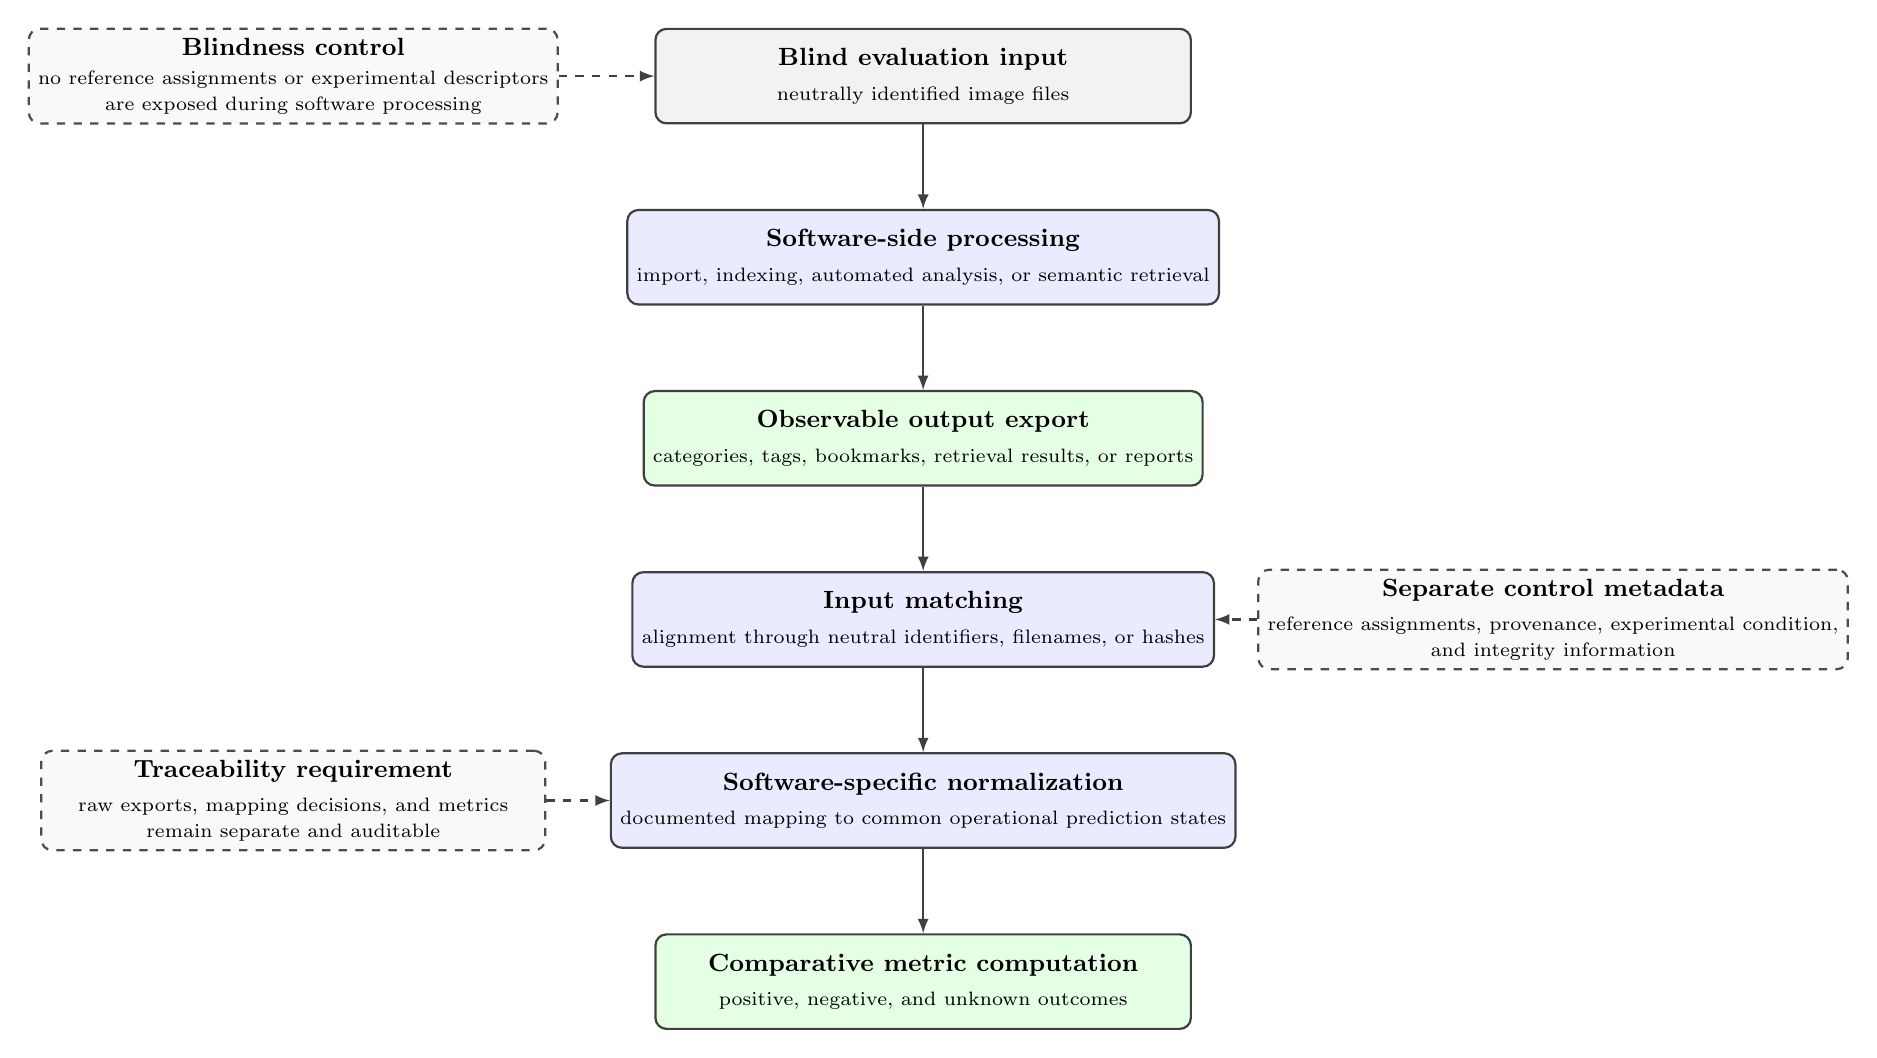
\begin{tikzpicture}[
>=latex,
font=\small,
block/.style={
rectangle,
rounded corners,
draw=black!75,
thick,
align=center,
minimum height=1.20cm,
minimum width=6.8cm,
fill=gray!10
},
process/.style={
rectangle,
rounded corners,
draw=black!75,
thick,
align=center,
minimum height=1.20cm,
minimum width=6.8cm,
fill=blue!8
},
output/.style={
rectangle,
rounded corners,
draw=black!75,
thick,
align=center,
minimum height=1.20cm,
minimum width=6.8cm,
fill=green!10
},
note/.style={
rectangle,
rounded corners,
draw=black!70,
dashed,
thick,
align=center,
minimum height=1.15cm,
minimum width=6.4cm,
fill=gray!5
},
arrow/.style={
->,
thick,
draw=black!75
},
dashedarrow/.style={
->,
thick,
dashed,
draw=black!75
}
]

\node[block] (blind) at (0,0)
{\shortstack{
\textbf{Blind evaluation input}\\[1mm]
\scriptsize neutrally identified image files
}};

\node[process] (processing) at (0,-2.3)
{\shortstack{
\textbf{Software-side processing}\\[1mm]
\scriptsize import, indexing, automated analysis, or semantic retrieval
}};

\node[output] (export) at (0,-4.6)
{\shortstack{
\textbf{Observable output export}\\[1mm]
\scriptsize categories, tags, bookmarks, retrieval results, or reports
}};

\node[process] (matching) at (0,-6.9)
{\shortstack{
\textbf{Input matching}\\[1mm]
\scriptsize alignment through neutral identifiers, filenames, or hashes
}};

\node[process] (normalization) at (0,-9.2)
{\shortstack{
\textbf{Software-specific normalization}\\[1mm]
\scriptsize documented mapping to common operational prediction states
}};

\node[output] (metrics) at (0,-11.5)
{\shortstack{
\textbf{Comparative metric computation}\\[1mm]
\scriptsize positive, negative, and unknown outcomes
}};

\node[note] (blindness) at (-8.0,0)
{\shortstack{
\textbf{Blindness control}\\[1mm]
\scriptsize no reference assignments or experimental descriptors\\
\scriptsize are exposed during software processing
}};

\node[note] (metadata) at (8.0,-6.9)
{\shortstack{
\textbf{Separate control metadata}\\[1mm]
\scriptsize reference assignments, provenance, experimental condition,\\
\scriptsize and integrity information
}};

\node[note] (traceability) at (-8.0,-9.2)
{\shortstack{
\textbf{Traceability requirement}\\[1mm]
\scriptsize raw exports, mapping decisions, and metrics\\
\scriptsize remain separate and auditable
}};

\draw[arrow] (blind) -- (processing);
\draw[arrow] (processing) -- (export);
\draw[arrow] (export) -- (matching);
\draw[arrow] (matching) -- (normalization);
\draw[arrow] (normalization) -- (metrics);

\draw[dashedarrow] (blindness.east) -- (blind.west);
\draw[dashedarrow] (metadata.west) -- (matching.east);
\draw[dashedarrow] (traceability.east) -- (normalization.west);

\end{tikzpicture}%
}
\caption[Black-box software evaluation workflow]{Black-box software evaluation
workflow. Neutrally identified inputs are processed without access to reference
operational assignments or experimental descriptors. Observable outputs are
subsequently matched to the control metadata, normalized through documented
software-specific rules, and converted into common operational prediction
states}
\label{fig:methodology-forensic-tool-workflow}
\end{figure}


% ─────────────────────────────────────────────────────────────────────────────
\section{Evaluation Metrics}
\label{sec:methodology-evaluation-metrics}
% ─────────────────────────────────────────────────────────────────────────────

The \gls{fairlab} metric framework evaluates three complementary dimensions of
operational robustness: binary classification performance under clean
conditions, robustness under adversarial and anti-forensic conditions, and
system behavior on \gls{ood} inputs. The framework also supports the evaluation
of selected black-box software systems after their heterogeneous outputs have
been normalized into common operational prediction states.

The objective is not limited to aggregate classification accuracy. In forensic
visual triage, different error types may have different operational
consequences. A false negative on a \texttt{weapon} sample may prevent
target-category content from being prioritized for detailed review. A false
positive may instead increase the volume of non-target material submitted to
the analyst.

The evaluation framework therefore combines conventional classification
metrics with condition-specific robustness indicators and operationally
oriented error measures. Binary metrics are computed separately for clean,
adversarial, and anti-forensic conditions. The \gls{ood} branch is evaluated
through separate behavioral indicators and is not integrated into the binary
confusion matrix.

The protocol does not adopt \gls{auroc} as a central metric. Although
score-based measures are widely used in supervised \gls{ml}, their consistent
application requires comparable continuous outputs across the evaluated
systems. The proxy models expose continuous prediction outputs, whereas the
selected black-box software systems may provide only categorical labels,
semantic tags, bookmarks, retrieval results, or system-specific scores whose
meaning and calibration cannot be independently verified.

The metric framework consequently prioritizes measures that can be derived
consistently from both inspectable models and normalized black-box outputs. This
choice does not imply a theoretical limitation of \gls{auroc} or other
score-based metrics. It reflects the operational requirement to compare
heterogeneous systems without assuming that their output scores have equivalent
meaning or calibration.

For the binary classification task, the principal metrics are accuracy,
balanced accuracy, precision, recall, F1-score, and the confusion matrix.
Class-specific interpretation is required because aggregate performance may
conceal asymmetric error behavior between the \texttt{weapon} and
\texttt{non\_weapon} classes.

Let \(TP\), \(TN\), \(FP\), and \(FN\) denote the numbers of true positives,
true negatives, false positives, and false negatives, respectively. Accuracy is
defined as:

\begin{equation}
\mathrm{Accuracy}
=
\frac{TP + TN}{TP + TN + FP + FN}
\end{equation}

Recall for the positive \texttt{weapon} class is defined as:

\begin{equation}
\mathrm{Recall}_{\text{\texttt{weapon}}}
=
\frac{TP}{TP + FN}
\end{equation}

The corresponding false-negative rate is:

\begin{equation}
\mathrm{FNR}_{\text{\texttt{weapon}}}
=
\frac{FN}{TP + FN}
\end{equation}

The false-positive rate is:

\begin{equation}
\mathrm{FPR}
=
\frac{FP}{FP + TN}
\end{equation}

Balanced accuracy accounts for performance on both operational classes:

\begin{equation}
\mathrm{Balanced\ Accuracy}
=
\frac{1}{2}
\left(
\frac{TP}{TP + FN}
+
\frac{TN}{TN + FP}
\right)
\end{equation}

Precision and F1-score are defined as:

\begin{equation}
\mathrm{Precision}
=
\frac{TP}{TP + FP}
\end{equation}

\begin{equation}
\mathrm{F1}
=
2
\frac{
\mathrm{Precision}
\cdot
\mathrm{Recall}_{\text{\texttt{weapon}}}
}{
\mathrm{Precision}
+
\mathrm{Recall}_{\text{\texttt{weapon}}}
}
\end{equation}

Robustness under manipulated conditions is evaluated by comparing the
prediction obtained for each perturbed artifact with both the corresponding
clean prediction and the reference operational class. This paired design makes
it possible to distinguish errors already present under clean conditions from
errors introduced after perturbation.

For a given perturbation condition \(p\), the accuracy drop is defined as:

\begin{equation}
\Delta \mathrm{Accuracy}_{p}
=
\mathrm{Accuracy}_{\mathrm{clean}}
-
\mathrm{Accuracy}_{p}
\end{equation}

Positive values indicate degradation relative to the clean baseline. Zero or
negative values indicate no measured degradation under the specific evaluated
condition and must not be interpreted as evidence of general robustness.

Let \(\mathcal{C}_{\mathrm{clean}}\) denote the set of samples classified
correctly under the clean condition. The induced error rate for condition \(p\)
is defined as:

\begin{equation}
\mathrm{InducedErrorRate}_{p}
=
\frac{
\left|
\left\{
i \in \mathcal{C}_{\mathrm{clean}}
:
\hat{y}^{(p)}_{i} \neq y_{i}
\right\}
\right|
}{
\left|
\mathcal{C}_{\mathrm{clean}}
\right|
}
\end{equation}

The numerator is the induced error count. For model-dependent adversarial
conditions, this rate may also be reported as the attack success rate because
it measures the proportion of clean-correct samples rendered incorrect by the
attack. Samples already misclassified under clean conditions do not contribute
to this quantity.

Particular attention is given to the transition:

\begin{equation}
\text{\texttt{weapon}}
\rightarrow
\text{\texttt{non\_weapon}}
\end{equation}

because it represents the loss of a positive detection for target-category
content. The reverse transition:

\begin{equation}
\text{\texttt{non\_weapon}}
\rightarrow
\text{\texttt{weapon}}
\end{equation}

is also measured because it may increase the volume of non-target content
prioritized for human review.

When continuous proxy-model outputs are available, the analysis also considers
the mean maximum predicted-class probability and its variation relative to the
corresponding clean condition. These quantities are used exclusively as
diagnostic intra-model indicators. They are not interpreted as calibrated
probabilities and must not be compared directly across different proxy
architectures.

For each proxy model and manipulated condition, the confidence shift is defined
as:

\begin{equation}
\Delta c
=
c_{\mathrm{perturbed}}
-
c_{\mathrm{clean}},
\end{equation}

where \(c\) denotes the maximum predicted-class probability. The value does not
necessarily correspond to the probability assigned to the reference operational
class.

The \gls{ood} evaluation remains conceptually separate from the binary
classification task. The \gls{ood} samples are not treated as a third
supervised class, and binary or multiclass accuracy is therefore not computed
for this branch.

Instead, the protocol characterizes how frequently \gls{ood} inputs are
assigned to the known operational classes. The principal indicators include:

\begin{itemize}
\item the proportion of \gls{ood} inputs assigned to
\texttt{weapon};

\item the proportion of \gls{ood} inputs assigned to
\texttt{non\_weapon};

\item the mean maximum predicted-class probability for proxy models;

\item the proportion of proxy-model predictions whose maximum probability
exceeds a predefined high-confidence threshold;

\item the proportion of unknown outputs, when such a state is exposed after
normalization of black-box software outputs.
\end{itemize}

The \gls{ood} weapon flag rate is defined as:

\begin{equation}
\mathrm{WeaponFlagRate}_{\mathrm{OOD}}
=
\frac{
N_{\mathrm{OOD}\rightarrow\text{\texttt{weapon}}}
}{
N_{\mathrm{OOD}}
}
\end{equation}

This measure describes the operational tendency of a system to map
distributionally different inputs to the target class. It does not represent a
conventional false-positive rate because the \gls{ood} inputs do not belong to
the supervised negative class. It also does not, by itself, establish that an
individual \gls{ood} assignment is semantically correct, incorrect, relevant,
or irrelevant.

Confidence-based \gls{ood} indicators are available only for the proxy models.
They remain diagnostic intra-model quantities and are not compared as calibrated
probabilities across architectures. The selected black-box software systems do
not expose homogeneous confidence values suitable for equivalent analysis.

The evaluation of black-box software systems is based on normalized observable
outputs. The common normalization framework distinguishes among positive
detection, no target detection, and \texttt{unknown}. The
\texttt{unknown} state includes missing, ambiguous, unsupported, unmapped, or
otherwise non-interpretable outputs.

Only matched records with interpretable positive or negative normalized
decisions contribute to the conventional binary confusion matrix. An unknown
output must not be forced into either the positive or negative class.

For samples whose reference operational class is \texttt{weapon}, an
interpretable no-target decision constitutes a false negative. In a separate
risk-oriented analysis, an unknown output may also be counted as an operational
miss because the target category was not surfaced. However, this supplementary
count must remain distinct from the conventional false-negative rate, and the
unknown outcomes must remain separately reportable.

For samples whose reference operational class is \texttt{non\_weapon}, an
interpretable target-related output constitutes a false positive. Unknown
outputs are not automatically treated as false positives because they do not
represent an explicit target detection.

For the selected black-box software systems, the protocol therefore considers:

\begin{itemize}
\item matching rate between exported outputs and bundle inputs;
\item true-positive and false-negative counts on interpretable records;
\item true-negative and false-positive counts on interpretable records;
\item weapon recall;
\item weapon false-negative rate;
\item false-positive rate;
\item accuracy and balanced accuracy, where the normalized outputs permit
their computation;
\item unknown output count and rate;
\item system-specific not-detected or uncategorized rates, where exposed;
\item supplementary operational miss counts, where explicitly defined.
\end{itemize}

The matching rate is a technical coverage measure rather than a classification
metric. It records the proportion of submitted bundle inputs for which a
corresponding software output can be identified:

\begin{equation}
\mathrm{MatchingRate}
=
\frac{
N_{\mathrm{matched}}
}{
N_{\mathrm{submitted}}
}
\end{equation}

The unknown output rate is defined as:

\begin{equation}
\mathrm{UnknownRate}
=
\frac{
N_{\mathrm{unknown}}
}{
N_{\mathrm{matched}}
}
\end{equation}

Unmatched inputs are represented through the matching rate and are not included
again in the numerator of the unknown rate. These technical coverage measures
are reported because incomplete matching or non-interpretable outputs may
affect the apparent performance of a black-box software system. They must not
be conflated with ordinary classification errors.

Table~\ref{tab:methodology-evaluation-metrics} summarizes the metric categories
adopted in the protocol.

\begin{table}[H]
\centering
\caption{Metric categories adopted in the evaluation protocol}
\label{tab:methodology-evaluation-metrics}
\begin{tabularx}{\textwidth}{@{}L{4.0cm}X@{}}
\toprule
\textbf{Category} &
\textbf{Metrics and operational meaning} \\
\midrule

Binary classification
&
Accuracy, balanced accuracy, precision, recall, F1-score, and confusion matrix
for the \texttt{weapon} and \texttt{non\_weapon} classes. \\

Robustness under manipulation
&
Clean and perturbed accuracy, accuracy drop, induced error count and rate,
prediction transitions, and intra-model confidence variation when available. \\

Critical operational errors
&
False negatives on \texttt{weapon} samples and false positives on
\texttt{non\_weapon} samples, interpreted according to their different effects
on forensic prioritization and review workload. \\

\gls{ood} behavior
&
Weapon flag rate, in-domain assignment distribution, and proxy-model
confidence indicators. The branch remains excluded from binary classification
metrics. \\

Black-box software coverage
&
Matching rate, unknown output count and rate, and system-specific missing,
not-detected, or uncategorized states. \\

Black-box classification behavior
&
True positives, false negatives, false positives, true negatives, weapon recall,
weapon false-negative rate, false-positive rate, accuracy, and balanced accuracy
computed on interpretable normalized outputs where applicable. \\

Supplementary operational-risk analysis
&
Unknown outcomes on \texttt{weapon} samples may be included in a separately
reported operational miss count without being recoded as conventional false
negatives. \\

\bottomrule
\end{tabularx}
\end{table}

Figure~\ref{fig:methodology-metric-layers} summarizes the metric framework
across the two complementary evaluation levels and the distinct binary,
manipulated-input, \gls{ood}, and coverage analyses.

\begin{figure}[H]
\centering
\resizebox{0.98\textwidth}{!}{%
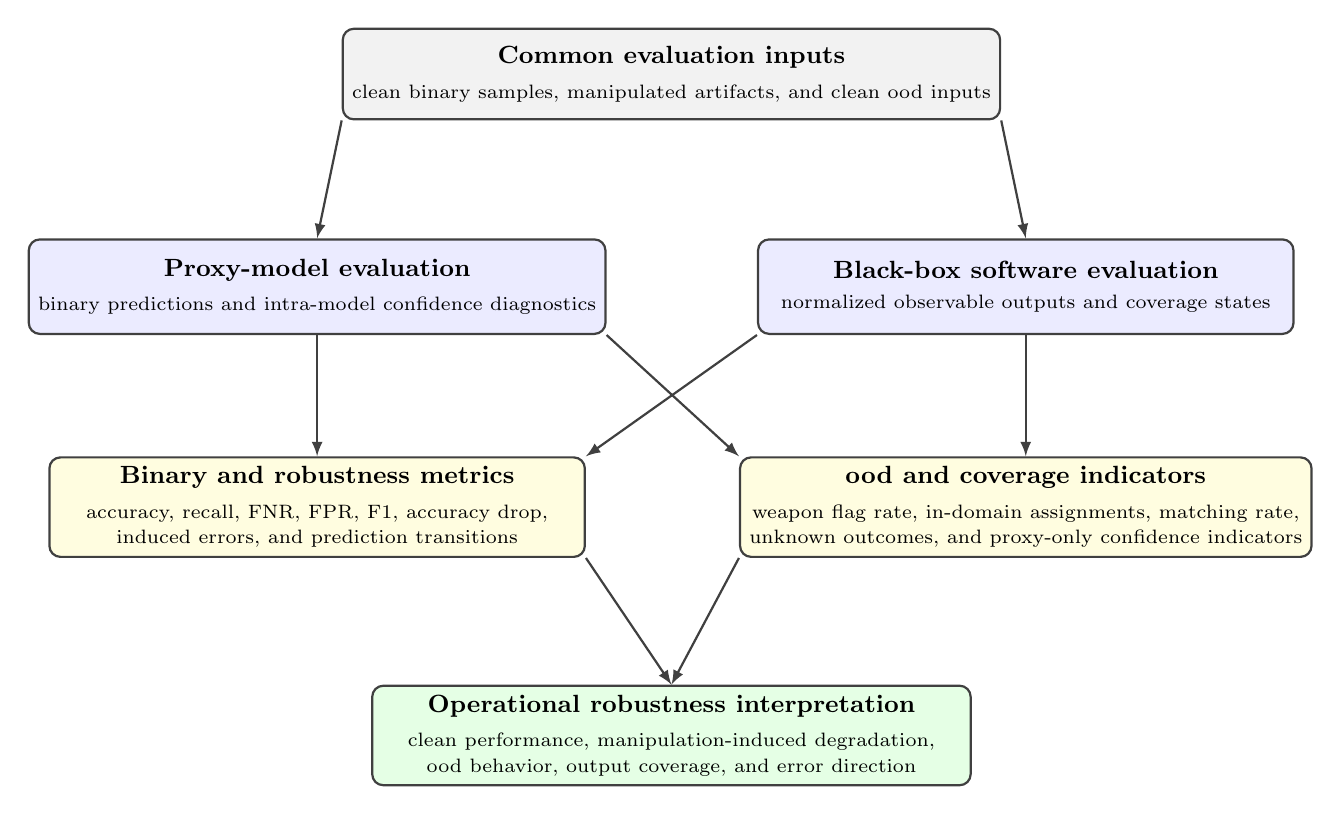
\begin{tikzpicture}[
>=latex,
font=\small,
block/.style={
rectangle,
rounded corners,
draw=black!75,
thick,
align=center,
minimum height=1.15cm,
minimum width=7.2cm,
fill=gray!10
},
eval/.style={
rectangle,
rounded corners,
draw=black!75,
thick,
align=center,
minimum height=1.20cm,
minimum width=6.8cm,
fill=blue!8
},
metric/.style={
rectangle,
rounded corners,
draw=black!75,
thick,
align=center,
minimum height=1.20cm,
minimum width=6.8cm,
fill=yellow!12
},
output/.style={
rectangle,
rounded corners,
draw=black!75,
thick,
align=center,
minimum height=1.20cm,
minimum width=7.6cm,
fill=green!10
},
arrow/.style={
->,
thick,
draw=black!75
}
]

\node[block] (inputs) at (0,0)
{\shortstack{
\textbf{Common evaluation inputs}\\[1mm]
\scriptsize clean binary samples, manipulated artifacts, and clean
\gls{ood} inputs
}};

\node[eval] (proxy) at (-4.5,-2.7)
{\shortstack{
\textbf{Proxy-model evaluation}\\[1mm]
\scriptsize binary predictions and intra-model confidence diagnostics
}};

\node[eval] (blackbox) at (4.5,-2.7)
{\shortstack{
\textbf{Black-box software evaluation}\\[1mm]
\scriptsize normalized observable outputs and coverage states
}};

\node[metric] (binary) at (-4.5,-5.5)
{\shortstack{
\textbf{Binary and robustness metrics}\\[1mm]
\scriptsize accuracy, recall, FNR, FPR, F1, accuracy drop,\\
\scriptsize induced errors, and prediction transitions
}};

\node[metric] (oodcoverage) at (4.5,-5.5)
{\shortstack{
\textbf{\gls{ood} and coverage indicators}\\[1mm]
\scriptsize weapon flag rate, in-domain assignments, matching rate,\\
\scriptsize unknown outcomes, and proxy-only confidence indicators
}};

\node[output] (interpretation) at (0,-8.4)
{\shortstack{
\textbf{Operational robustness interpretation}\\[1mm]
\scriptsize clean performance, manipulation-induced degradation,\\
\scriptsize \gls{ood} behavior, output coverage, and error direction
}};

\draw[arrow] (inputs.south west) -- (proxy.north);
\draw[arrow] (inputs.south east) -- (blackbox.north);

\draw[arrow] (proxy.south) -- (binary.north);
\draw[arrow] (proxy.south east) -- (oodcoverage.north west);

\draw[arrow] (blackbox.south west) -- (binary.north east);
\draw[arrow] (blackbox.south) -- (oodcoverage.north);

\draw[arrow] (binary.south east) -- (interpretation.north);
\draw[arrow] (oodcoverage.south west) -- (interpretation.north);

\end{tikzpicture}%
}
\caption[Metric framework]{Metric framework. Condition-specific binary,
robustness, \gls{ood}, and coverage indicators are computed across the
proxy-model and black-box evaluation levels and integrated only during the
operational interpretation}
\label{fig:methodology-metric-layers}
\end{figure}

The metrics do not replace human review or establish that a software system is
reliable across all forensic scenarios. Their function is to identify the
conditions under which automated support may fail to surface target-category
content, increase the review workload, or produce unstable or operationally
consequential outputs on manipulated or distributionally different inputs.


% ─────────────────────────────────────────────────────────────────────────────
\section{Explainability Approach}
\label{sec:methodology-explainability}
% ─────────────────────────────────────────────────────────────────────────────

The \gls{xai} component of the \gls{fairlab} methodology serves an exclusively
diagnostic and qualitative function. It complements quantitative robustness
metrics by supporting the examination of selected cases in which the behavior
of an inspectable proxy classification model is operationally or
methodologically relevant.

Explainability outputs are not treated as stand-alone evidence, definitive
explanations of algorithmic decisions, or demonstrations of model reliability.
Their purpose is to provide diagnostic information about the attribution
patterns associated with a selected model output and to support the formulation
of hypotheses regarding changes in model behavior across clean, adversarial,
anti-forensic, and \gls{ood} conditions.

In the present research design, the explainability analysis is restricted to
one selected fully inspectable proxy model. The adopted technique must therefore
be compatible with the model architecture, weights, preprocessing procedure,
and inference pipeline. Depending on the selected method, access may also be
required to gradients, intermediate activations, or other differentiable model
components.

The same internal attribution analysis cannot be applied directly to the
selected black-box or near-black-box software systems. Their internal model
architectures, gradients, representations, decision thresholds, and scoring
procedures are not accessible. Comparisons involving these systems are
therefore limited to their observable and normalized outputs. Such outputs must
not be interpreted as explanations of the internal decision processes that
produced them.

The explainability methodology adopts a case-study approach rather than an
aggregate evaluation strategy. Representative samples are selected according to
predefined diagnostic criteria. The objective is not to estimate model
performance from a limited number of visualizations, but to examine specific
behaviors that cannot be fully characterized through aggregate metrics alone.

Relevant case categories include:

\begin{itemize}
\item a correctly classified clean sample used as a qualitative reference;

\item a clean sample associated with an operationally relevant
classification error;

\item a high-confidence \gls{ood} assignment to an in-domain operational
class;

\item a clean-correct sample rendered incorrect by an anti-forensic
transformation;

\item a clean-correct sample rendered incorrect by a model-dependent
adversarial perturbation, particularly when the resulting prediction
retains high model confidence.
\end{itemize}

High-confidence criteria are applied only within the selected proxy model. They
serve as diagnostic case-selection indicators and must not be interpreted as
calibrated probabilities or compared directly with confidence values from other
architectures or software systems.

Table~\ref{tab:methodology-xai-case-selection} summarizes the diagnostic
function of these case categories.

\begin{table}[H]
\centering
\caption{Case-selection criteria for explainability analysis}
\label{tab:methodology-xai-case-selection}
\begin{tabularx}{\textwidth}{@{}L{4.4cm}X@{}}
\toprule
\textbf{Case category} &
\textbf{Diagnostic function} \\
\midrule

Correctly classified clean reference
&
Provide a qualitative reference for examining whether the attribution pattern
is associated with visually relevant regions under an unmanipulated condition.
\\

Clean classification error
&
Examine an error already present under the clean condition and determine
whether the attribution pattern appears localized, diffuse, partial, or
associated with contextual image regions. \\

High-confidence \gls{ood} assignment
&
Examine the attribution pattern associated with an in-domain assignment
produced for a distributionally different input. The assignment is treated as
an operational behavior rather than as an ordinary supervised error. \\

Anti-forensic induced error
&
Examine whether an operationally plausible image transformation is associated
with a change in the attribution pattern and the resulting predicted class. \\

Adversarially induced error
&
Examine the attribution pattern associated with an incorrect prediction
produced after a model-dependent adversarial perturbation, including cases in
which the model output remains highly confident. \\

\bottomrule
\end{tabularx}
\end{table}

Case selection must remain traceable to the corresponding prediction records,
source samples, experimental conditions, and model configurations. Each
explainability artifact should therefore be associated with the evaluated
sample, the model and checkpoint used for inference, the predicted class, the
reference operational class, the evaluation condition, and the rationale for
case selection.

The methodology does not prescribe a single explainability technique for every
possible implementation of the protocol. Gradient-based attribution,
activation-based visualization, local surrogate methods, and other
feature-attribution approaches may be considered, provided that their
assumptions and limitations are compatible with the selected model and the
research questions under examination. The specific technique and configuration
adopted in this thesis are reported in
Chapter~\ref{chap:implementation}.

The adopted explainability procedure should satisfy the following requirements:

\begin{itemize}
\item compatibility with the selected inspectable proxy model;
\item explicit documentation of the attribution target and reference
baseline, where required by the method;
\item reproducibility of the attribution procedure;
\item consistent application across the selected clean and manipulated
cases;
\item traceability to the model checkpoint, input sample, and prediction
record;
\item production of outputs that can be interpreted without being presented
as definitive causal explanations.
\end{itemize}

Attribution maps and related visualizations must be interpreted cautiously.
They characterize the relationship between input features and a selected model
output under the assumptions of the adopted explainability method. They do not
establish that the highlighted regions reproduce the model's internal
reasoning, nor do they demonstrate that the resulting prediction is correct,
reliable, or forensically valid.

When the adopted method provides completeness, approximation, or convergence
diagnostics, these quantities should be documented and considered during
interpretation. They constitute validation aids rather than automatic evidence
that an attribution is complete or reliable. No strict convergence claim should
be made unless it is supported by the recorded diagnostic values and the
adopted acceptance criterion.

The explainability analysis must also remain distinct from the quantitative
robustness assessment. Classification metrics measure the frequency, magnitude,
and direction of observed errors across the experimental corpus. Explainability
instead supports the qualitative examination of selected examples and the
interpretation of possible changes in attribution patterns.

Within the \gls{fairlab} protocol, \gls{xai} therefore acts as a supporting
diagnostic layer. It contributes to the interpretation of representative model
decisions and failure cases while preserving the distinction among technical
attribution, experimental robustness evaluation, and the evidentiary assessment
performed by a human forensic analyst.


% ─────────────────────────────────────────────────────────────────────────────
\section{Traceability and Reproducibility Controls}
\label{sec:methodology-traceability-controls}
% ─────────────────────────────────────────────────────────────────────────────

Traceability is a cross-cutting requirement of the entire \gls{fairlab}
protocol. It applies not only to dataset construction, but to every stage of the
experimental workflow, including technical preparation, human-in-the-loop
review, dataset freezing, partition generation, proxy-model training,
perturbation generation, bundle construction, black-box software evaluation,
metric computation, and \gls{xai} analysis.

Consistent with established \gls{df} principles, each processing step that
creates or modifies an experimental file must be documented so that the
relationships among the original sample, any derived artifact, the
corresponding model or software output, and the final experimental result can
be reconstructed
\cite{casey2011digital,nist2006guide,iso27037}.

The traceability framework relies on stable identifiers, integrity information,
structured provenance records, and explicit associations among experimental
inputs, derived artifacts, configurations, and outputs. Each sample must remain
identifiable throughout its complete lifecycle, even when its filename,
encoding, directory location, or visual representation changes.

The methodology distinguishes among four complementary traceability elements:

\begin{enumerate}
\item \textit{sample identity}, which establishes a stable reference to the
original image;

\item \textit{artifact lineage}, which records the relationship between an
original sample and any derived adversarial, anti-forensic, blind-bundle, or
explainability artifact;

\item \textit{experimental context}, which associates each input or derived
artifact with its reference operational assignment, partition, model
configuration, perturbation condition, and evaluation branch;

\item \textit{output provenance}, which connects model predictions,
software exports, normalization decisions, metrics, and qualitative case
studies to the corresponding evaluation input.
\end{enumerate}

Integrity verification should be based on cryptographic identifiers or other
mechanisms capable of detecting unintended changes to the experimental files.
The methodology does not prescribe a specific hashing algorithm. The selected
mechanism must nevertheless be documented and applied consistently across the
relevant stages of the pipeline.

Additional identifiers may be retained when required for interoperability with
selected black-box software systems. Such auxiliary identifiers must not
replace the primary integrity mechanism unless their security and
collision-resistance properties are appropriate for that role.

Traceability records should be progressive. Each stage should preserve the
identifiers inherited from the preceding stage and add only the information
required to describe the newly created artifact, configuration, or experimental
condition. This approach enables the lifecycle of each sample to be
reconstructed without relying exclusively on directory structures or
filenames.

Table~\ref{tab:methodology-traceability-artifacts} summarizes the principal
categories of traceability records required by the methodology.

\begin{table}[H]
\centering
\caption{Principal traceability records across the FAIRLab protocol}
\label{tab:methodology-traceability-artifacts}
\begin{tabularx}{\textwidth}{@{}L{4.2cm}X@{}}
\toprule
\textbf{Record category} &
\textbf{Role in traceability} \\
\midrule

Technical preparation records
&
Document sample identity, provenance, technical validity, and integrity
information for the candidate image pool. \\

Human-review records
&
Associate each candidate sample with its review status, operational assignment,
exclusion disposition, and supporting notes. \\

Frozen-dataset records
&
Define the stable experimental corpus and preserve the reference operational
assignments used in the subsequent phases. \\

Partition records
&
Associate each sample with its binary or \gls{ood} evaluation branch and, where
applicable, its experimental fold. \\

Model records
&
Document model architecture, training configuration, class mapping, checkpoint
identity, and the relationship between each checkpoint and its training
partitions. \\

Derived-artifact records
&
Link adversarial and anti-forensic artifacts to the corresponding clean sample,
generation condition, parameters, and model configuration when applicable. \\

Evaluation-bundle records
&
Map neutral blind identifiers to the corresponding source sample, reference
operational assignment, experimental condition, and integrity information. \\

Prediction and normalization records
&
Connect proxy-model predictions and observable software outputs to the evaluated
input and document any matching, recoding, or mapping decision. \\

Metric and explainability records
&
Associate quantitative results and qualitative case studies with the underlying
samples, model checkpoints, software configurations, and experimental
conditions. Explainability records refer only to the selected inspectable proxy
model. \\

\bottomrule
\end{tabularx}
\end{table}

The minimum traceability chain must make it possible to move in both directions:
from an original sample to its evaluation inputs, derived artifacts, and
experimental outputs, and from a reported result back to the exact input,
configuration, and processing conditions that produced it.

Figure~\ref{fig:methodology-traceability-chain} summarizes this general
traceability chain.

\begin{figure}[H]
\centering
\resizebox{0.96\textwidth}{!}{%
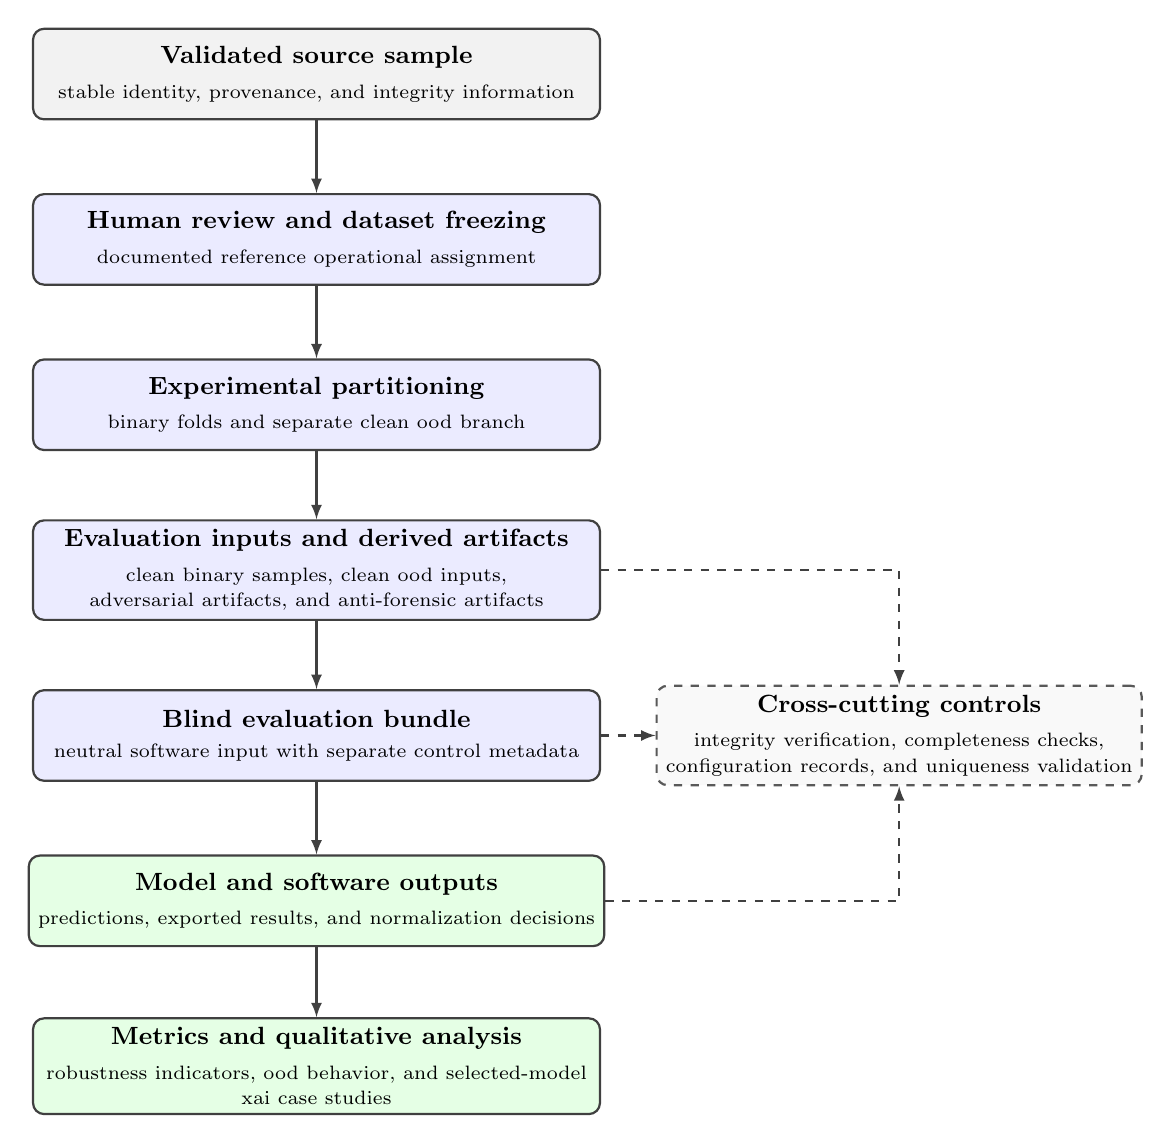
\begin{tikzpicture}[
>=latex,
font=\small,
block/.style={
rectangle,
rounded corners,
draw=black!75,
thick,
align=center,
minimum height=1.15cm,
minimum width=7.2cm,
fill=gray!10
},
process/.style={
rectangle,
rounded corners,
draw=black!75,
thick,
align=center,
minimum height=1.15cm,
minimum width=7.2cm,
fill=blue!8
},
output/.style={
rectangle,
rounded corners,
draw=black!75,
thick,
align=center,
minimum height=1.15cm,
minimum width=7.2cm,
fill=green!10
},
note/.style={
rectangle,
rounded corners,
draw=black!65,
dashed,
thick,
align=center,
minimum height=1.05cm,
minimum width=6.0cm,
fill=gray!5
},
arrow/.style={
->,
thick,
draw=black!75
},
dashedarrow/.style={
->,
thick,
dashed,
draw=black!75
}
]

\node[block] (source) at (0,0)
{\shortstack{
\textbf{Validated source sample}\\[1mm]
\scriptsize stable identity, provenance, and integrity information
}};

\node[process] (review) at (0,-2.1)
{\shortstack{
\textbf{Human review and dataset freezing}\\[1mm]
\scriptsize documented reference operational assignment
}};

\node[process] (partition) at (0,-4.2)
{\shortstack{
\textbf{Experimental partitioning}\\[1mm]
\scriptsize binary folds and separate clean \gls{ood} branch
}};

\node[process] (evaluationinputs) at (0,-6.3)
{\shortstack{
\textbf{Evaluation inputs and derived artifacts}\\[1mm]
\scriptsize clean binary samples, clean \gls{ood} inputs,\\
\scriptsize adversarial artifacts, and anti-forensic artifacts
}};

\node[process] (bundle) at (0,-8.4)
{\shortstack{
\textbf{Blind evaluation bundle}\\[1mm]
\scriptsize neutral software input with separate control metadata
}};

\node[output] (predictions) at (0,-10.5)
{\shortstack{
\textbf{Model and software outputs}\\[1mm]
\scriptsize predictions, exported results, and normalization decisions
}};

\node[output] (analysis) at (0,-12.6)
{\shortstack{
\textbf{Metrics and qualitative analysis}\\[1mm]
\scriptsize robustness indicators, \gls{ood} behavior, and selected-model\\
\scriptsize \gls{xai} case studies
}};

\node[note] (controls) at (7.4,-8.4)
{\shortstack{
\textbf{Cross-cutting controls}\\[1mm]
\scriptsize integrity verification, completeness checks,\\
\scriptsize configuration records, and uniqueness validation
}};

\draw[arrow] (source) -- (review);
\draw[arrow] (review) -- (partition);
\draw[arrow] (partition) -- (evaluationinputs);
\draw[arrow] (evaluationinputs) -- (bundle);
\draw[arrow] (bundle) -- (predictions);
\draw[arrow] (predictions) -- (analysis);

\draw[dashedarrow] (evaluationinputs.east) -| (controls.north);
\draw[dashedarrow] (bundle.east) -- (controls.west);
\draw[dashedarrow] (predictions.east) -| (controls.south);

\end{tikzpicture}%
}
\caption[Traceability chain across the FAIRLab protocol]{Traceability chain
across the FAIRLab protocol. Stable identifiers, provenance information,
integrity controls, and structured records preserve the relationships among
source samples, evaluation inputs, derived artifacts, observable outputs, and
final analyses}
\label{fig:methodology-traceability-chain}
\end{figure}

Reproducibility requires more than the availability of source code. The
experimental configuration must be documented in sufficient detail to recreate
the relevant processing conditions. This documentation should include the
dataset version, partitioning strategy, randomization controls, model
configuration, preprocessing rules, perturbation parameters, software version,
enabled functionality, normalization rules, and metric definitions.

Where randomness affects dataset partitioning, model initialization,
optimization, perturbation generation, or case selection, the relevant random
state or deterministic procedure must be recorded. Deterministic execution is
preferred when it does not conflict with the intended experimental design.

Model artifacts must be associated with the training partitions and
configuration that produced them. In fold-aware evaluation, the proxy-model
checkpoint used to evaluate a held-out binary sample, or to generate a
model-dependent adversarial artifact from that sample, must not have been
trained on the sample itself. This constraint reduces the risk of information
leakage and supports valid interpretation of the resulting robustness
measurements.

Generated adversarial and anti-forensic artifacts must preserve their
relationships with the corresponding clean inputs. Model-dependent adversarial
artifacts must additionally identify the relevant source model and
fold-specific checkpoint. This information is required to distinguish direct
source-model evaluation from cross-model and black-box transfer evaluation.

Model-agnostic adversarial-style and anti-forensic artifacts do not originate
from a designated source model. Their records must instead preserve the shared
generation condition and applied configuration so that responses can be
compared across proxy models and selected black-box software systems without
describing the comparison as transferability.

The blind evaluation of selected black-box software systems introduces an
additional traceability requirement. Experimental metadata must remain separate
from the software input during processing, but must remain available after
export to support input matching, normalization, and metric computation.

The separation between blind inputs and control metadata must itself be
verifiable. The evaluation records should demonstrate that reference
operational assignments, perturbation names, fold allocations, model
identifiers, and other controlled experimental descriptors were not exposed
through filenames, paths, directory structures, or accompanying control files
during software processing.

Automated consistency controls should verify, where applicable:

\begin{itemize}
\item correspondence between expected and generated artifacts;
\item uniqueness of stable and derived identifiers;
\item integrity of generated files;
\item absence of missing or unresolved paths;
\item consistency among source records, derived artifacts, and evaluation
outputs;
\item completeness of software exports and normalized predictions;
\item separation between blind inputs and experimental metadata.
\end{itemize}

These controls establish the technical coherence of the experimental workflow.
They do not demonstrate classification correctness or operational robustness.
Their purpose is to ensure that the reported results derive from the intended
inputs, artifacts, and configurations rather than from undocumented
substitutions, incomplete runs, or incorrect associations.

Traceability and reproducibility must also be considered within the limitations
of black-box evaluation. Selected software systems may change across versions,
and their internal models, thresholds, or processing logic may remain
unavailable. Accordingly, reproducibility in this context concerns the
documented external configuration, submitted inputs, observable outputs, and
normalization procedures rather than the inaccessible internal inference
process.

The protocol therefore combines procedural reproducibility with artifact-level
traceability. Procedural reproducibility documents how the experiment can be
repeated, whereas artifact-level traceability makes it possible to verify which
specific inputs, models, software configurations, and derived files contributed
to each reported result.

The concrete implementation of these controls is documented in
Chapter~\ref{chap:implementation}, whereas the corresponding experimental
outcomes are reported in Chapter~\ref{chap:results}.
















